\chapter{Metodologia}
\label{cap:metodologia}
% --------------------------------------------------------------------------

Este capítulo detalha o rigor metodológico aplicado ao desenvolvimento, à aceleração neural e à validação do chassi primário auxético para nanossatélites CubeSat 1U. A pesquisa estrutura-se sobre uma abordagem computacional integrada que combina a análise dimensional celular, a modelagem multiescala por elementos de volume representativo (RVE), a síntese paramétrica B-Rep com restrições de Manufatura Aditiva (DfAM) e simulações elastodinâmicas de alta fidelidade em elementos finitos no ecossistema aberto (Code\_Aster e Gmsh Tet10 em ambiente Linux/WSL). O fluxo operacional está dividido em quatro fases sequenciais: (i) ancoragem constitutiva direta na liga aeroespacial AlSi10Mg e parametrização geométrica; (ii) modelagem de contorno e homogeneização assintótica; (iii) simulação dinâmica normatizada em código aberto e síntese do modelo substituto neural guiado por física (\textit{Physics-Guided ResNet}); e (iv) validação de alta ordem (\textit{Code\_Aster Ground Truth}) e integridade à fadiga estocástica.

\section{Princípio de similaridade mecânica, análise dimensional e limites de transferibilidade}
\label{sec:similaridade}

A formulação teórica de escala para metamateriais celulares fundamenta-se na Teoria da Similaridade Mecânica e na análise dimensional governada pelo Teorema Pi de Buckingham (NASA, 2016). Esse princípio estabelece que sistemas físicos governados pelos mesmos fenômenos constitutivos preservam relações dinâmicas invariantes quando os grupos adimensionais característicos são estritamente conservados.

No domínio dos metamateriais celulares e estruturas treliçadas, a variável adimensional governante primária é a densidade relativa ($\rho^{*}/\rho_s$), que define a fração de volume ocupada pelo material sólido e dita a rigidez elástica equivalente ($E^{*}/E_s$). De acordo com as leis fundamentais de Gibson e Ashby (1997), a relação constitutiva macroscópica para matrizes celulares dominadas por flexão é regida pela lei de potência formulada na Equação~\eqref{eq:pi1}:
\begin{equation}
  \Pi_1 = \frac{E^{*}}{E_s} = C \left( \frac{\rho^{*}}{\rho_s} \right)^{n}
  \label{eq:pi1}
\end{equation}
na qual $C$ e $n$ são constantes topológicas puras associadas à cinemática de deformação da célula unitária reentrante.

Para o comportamento elastodinâmico e o desacoplamento ressonante no veículo lançador, a formulação dimensional define o segundo grupo adimensional ($\Pi_2$), correlacionando a frequência natural fundamental ($f_n$), a dimensão característica macroscópica ($L$) e as propriedades mecânicas eficazes:
\begin{equation}
  \Pi_2 = f_n \cdot L \sqrt{\frac{\rho^{*}}{E^{*}}} = \text{constante} \quad \implies \quad f_n \propto \frac{1}{L} \sqrt{\frac{E^{*}}{\rho^{*}}}
  \label{eq:fn}
\end{equation}

Contudo, sob o rigor estrito da qualificação estrutural aeroespacial, é imperativo explicitar os limites físicos de validade dessa abordagem dimensional. Embora a similaridade elástica linear clássica governada por $\Pi_1$ e $\Pi_2$ forneça correlações consistentes para deformações estáticas e autovalores modais teóricos não amortecidos em meios homotéticos, ela configura uma \textbf{similaridade incompleta (\textit{incomplete similarity})} quando estendida à dinâmica estocástica de vibração aleatória e à integridade em fadiga. Existem divergências constitutivas intransponíveis entre domínios poliméricos (como termoplásticos impressos por FDM) e ligas metálicas aeroespaciais:
\begin{alineas}
  \item \textbf{amortecimento e dissipação interna de energia:} termoplásticos exibem comportamento viscoelástico pronunciado, com amortecimento interno fortemente dependente da taxa de deformação e temperatura ($\zeta_{\text{polímero}} \approx \num{0.03}$ a $\num{0.06}$, ou seja, $3\text{ a }6\%$), enquanto ligas metálicas aeroespaciais consolidadas por fusão a laser apresentam dissipação histerética muito inferior ($\zeta_{\text{AlSi10Mg}} \approx \num{0.005}$ a $\num{0.02}$, $0{,}5\text{ a }2\%$). Essa discrepância altera de forma radical o fator de amplificação dinâmica na ressonância ($Q = 1 / [2\zeta]$);
  \item \textbf{razão de rigidez e microestrutura celular:} a liga AlSi10Mg produzida por L-PBF exibe módulo de elasticidade cerca de 25 vezes superior ao de termoplásticos comerciais ($E_{\text{metal}} = \SI{68.0}{\giga\pascal}$ contra $E_{\text{polímero}} \approx \SI{2.5}{\giga\pascal}$ a $\SI{3.5}{\giga\pascal}$). Além disso, a microestrutura do metal solidificado por laser é formada por redes celulares eutéticas de silício finamente dispersas em matriz de alumínio, diferindo substancialmente da adesão térmica entre filamentos poliméricos;
  \item \textbf{sensibilidade a entalhes, porosidades térmicas e mecânica da fratura:} o processo L-PBF induz tensões residuais térmicas de tração decorrentes do ciclo térmico ultrarrápido de fusão/solidificação, além de microporosidades intrínsecas (defeitos de falta de fusão e poros de aprisionamento gasoso). Sob vibração aleatória estocástica, tais descontinuidades atuam como concentradores de tensão severos com mecanismo de propagação de trincas por fadiga de alto ciclo e fratura linear elástica frágil, ausentes na viscoelasticidade dúctil de polímeros.
\end{alineas}

Em face dessas distinções fenomenológicas, este trabalho descarta categoricamente qualquer tentativa de extrapolação empírica de respostas dinâmicas ou calibração de malha a partir de materiais plásticos. O emprego de modelos conceituais tridimensionais preliminares em filamento termoplástico (PLA) circunscreve-se estritamente à verificação física de empacotamento volumétrico e checagem dimensional de montagem (\textit{fit-check} virtual) nas interfaces dos trilhos do casulo lançador P-POD e placas de aviônica PC/104. Toda a modelagem constitutiva, o banco de dados de simulações elastodinâmicas e a qualificação espacial são ancorados de forma direta, unívoca e rigorosa nas propriedades da liga metálica de voo AlSi10Mg processada por L-PBF.

\section{Fases da metodologia}
\label{sec:fases}

\subsection{Ancoragem constitutiva na liga aeroespacial AlSi10Mg (L-PBF)}
\label{subsec:caracterizacao}

A primeira fase metodológica compreende a ancoragem constitutiva unívoca na liga aeroespacial AlSi10Mg aliviada termicamente ($300^\circ\text{C} / 2\text{ h}$), amplamente consolidada na indústria espacial para componentes estruturais fabricados por Fusão em Leito de Pó a Laser (L-PBF). Em conformidade com as normas internacionais de qualificação de materiais aeroespaciais e relatórios técnicos de caracterização aditiva (SLEJKO \textit{et al.}, 2023; KHAN; RICCIO, 2024), adotam-se as propriedades mecânicas canônicas listadas na Tabela~\ref{tab:propriedades-alsi10mg}.

\begin{table}[htb]
  \caption{Propriedades mecânicas e critérios de projeto da liga aeroespacial AlSi10Mg (L-PBF) com alívio térmico}
  \label{tab:propriedades-alsi10mg}
  \small
  \SingleSpacing
  \begin{tabularx}{\textwidth}{@{}>{\raggedright\arraybackslash}X >{\centering\arraybackslash}p{3.5cm} >{\centering\arraybackslash}p{4.0cm}@{}}
    \toprule
    \textbf{Propriedade termomecânica} & \textbf{Símbolo / Parâmetro} & \textbf{Valor adotado} \\
    \midrule
    Módulo de elasticidade longitudinal (Young) & $E$ & \SI{68.0}{\giga\pascal} \\
    Coeficiente de Poisson & $\nu$ & \num{0.33} \\
    Massa específica & $\rho$ & \SI{2670.0}{\kilo\gram\per\cubic\metre} \\
    Limite de escoamento convencional ($0{,}2\%$) & $\sigma_{\text{yield}}$ & \SI{230.0}{\mega\pascal} \\
    Limite de resistência à tração & $\sigma_{\text{ult}}$ & \SI{340.0}{\mega\pascal} \\
    Fator de segurança de qualificação (NASA GEVS) & $FS_{\text{yield}}$ & \num{1.25} \\
    Tensão admissível de projeto estocástico & $\sigma_{\text{adm}} = \sigma_{\text{yield}} / FS_{\text{yield}}$ & \SI{184.0}{\mega\pascal} \\
    Limiar de propagação de trincas por fadiga & $\Delta K_{th}$ & \SI{2.50}{\mega\pascal\sqrt{\metre}} \\
    \bottomrule
  \end{tabularx}
  \fonte{Elaborada pelo autor com base em Slejko \textit{et al.} (2023) e NASA (2013).}
\end{table}

No regime de pequenas deformações elásticas e vibração linear, o comportamento tridimensional do metal isotrópico contínuo é governado pela lei constitutiva generalizada de Hooke, expressa na Equação~\eqref{eq:hooke-3d}:
\begin{equation}
  \boldsymbol{\sigma} = \mathbf{C} : \boldsymbol{\varepsilon} = \lambda \operatorname{tr}(\boldsymbol{\varepsilon})\mathbf{I} + 2\mu\boldsymbol{\varepsilon}
  \label{eq:hooke-3d}
\end{equation}
na qual $\lambda$ e $\mu$ denotam os parâmetros elásticos de Lamé calculados a partir de $E$ e $\nu$:
\begin{equation}
  \lambda = \frac{E\,\nu}{(1+\nu)(1-2\nu)} = \SI{44.20}{\giga\pascal}, \qquad \mu = \frac{E}{2(1+\nu)} = G = \SI{25.56}{\giga\pascal}
  \label{eq:lame}
\end{equation}

Essa ancoragem direta nas constantes termomecânicas da liga metálica de voo elimina as incertezas e distorções constitutivas inerentes a extrapolações polímero-metal, assegurando que o espaço amostral do DoE, a inferência neural da ResNet e as margens de qualificação espacial da NASA GEVS reproduzam com alta fidelidade a física real do chassi primário de voo.

\subsection{Modelagem implícita e homogeneização assintótica}
\label{subsec:implicita}

A segunda fase da metodologia aborda a parametrização matemática e a redução computacional da estrutura celular. Cumpre explicitar a coexistência e os papéis complementares de duas representações geométricas no pipeline de desenvolvimento: a formulação implícita por superfícies de nível com base de Fourier (\textit{Fourier Level-Set}) representa o arcabouço teórico para a homogeneização analítica e o projeto de estruturas celulares com gradação funcional de densidade (\textit{Functionally Graded Lattices} -- FGL), viabilizando transições contínuas de densidade relativa; por sua vez, a síntese computacional em ambiente CAD via CadQuery/OpenCASCADE e a discretização por elementos finitos no Gmsh e Code\_Aster utilizam representação por contorno (\textit{Boundary Representation} -- B-Rep) governada pelo vetor explícito de parâmetros geométricos $\mathbf{x} = [\theta, t, l, h]^\top$.

No domínio analítico do \textit{Level-Set}, o domínio sólido $\Omega$ do metamaterial é definido pelo conjunto de pontos no espaço tridimensional delimitados pelo campo escalar contínuo $V(x,y,z)$, sujeito ao limiar de corte $t$:
\begin{equation}
  \Omega = \left\{ (x,y,z) \in \mathbb{R}^3 \;\middle|\; V(x,y,z) \le t \right\}, \qquad \partial\Omega = \left\{ (x,y,z) \in \mathbb{R}^3 \;\middle|\; V(x,y,z) = t \right\}
  \label{eq:iso}
\end{equation}
onde $\partial\Omega$ demarca a fronteira sólida externa da estrutura celular e o limiar $t$ modula diretamente a espessura média de parede e a densidade relativa local ($\rho^{*}/\rho_s$).

Para a célula unitária auxética reentrante tridimensional, cuja geometria paramétrica está apresentada na Figura~\ref{fig:celula-auxetica}, o campo de nível $V(x,y,z)$ é construído sobre uma base periódica de Fourier truncada de período cúbico $L$:
\begin{equation}
  \begin{aligned}
    V(x,y,z) ={}& \cos\!\left(\tfrac{2\pi x}{L}\right)\cos\!\left(\tfrac{2\pi y}{L}\right)
      + \cos\!\left(\tfrac{2\pi y}{L}\right)\cos\!\left(\tfrac{2\pi z}{L}\right)
      + \cos\!\left(\tfrac{2\pi z}{L}\right)\cos\!\left(\tfrac{2\pi x}{L}\right) \\
    & - \gamma \left[ \cos\!\left(\tfrac{2\pi x}{L}\right) + \cos\!\left(\tfrac{2\pi y}{L}\right) + \cos\!\left(\tfrac{2\pi z}{L}\right) \right]
  \end{aligned}
  \label{eq:fourier}
\end{equation}
onde o parâmetro $\gamma$ controla o grau de reentrância angular das paredes oblíquas, ditando a magnitude do coeficiente de Poisson negativo sob carregamento axial. A variação contínua da função de limiarização $t(x,y,z)$ possibilita a transição geométrica suave para uma Estrutura de Densidade Graduada (\textit{Functionally Graded Lattice} -- FGL), em estrita conformidade com as diretrizes de DfAM (KHAN; RICCIO, 2024).

Cumpre registrar com rigor conceitual que essa formulação analítica implícita baseada em superfícies de nível de Fourier atua nesta pesquisa estritamente como fundamentação teórica de referência contínua para o estado da arte em metamateriais e futuras expansões de otimização topológica inversa. Em contrapartida, toda a esteira computacional de síntese geométrica, checagens diagnósticas de fabricabilidade aditiva (DfAM), exportação no padrão industrial neutro STEP AP214 (ISO 10303-21) e discretização volumétrica de alta ordem no Gmsh adota deliberadamente a modelagem geométrica por contorno (\textit{Boundary Representation} -- B-Rep) governada pelo vetor paramétrico dimensional explícito $\mathbf{x} = [\theta, t, l, h]^\top$, detalhada na Seção~\ref{subsec:opencad-dfam}. Essa escolha de engenharia garante geometria analítica exata, previne artefatos espúrios de discretização de malha superficial e viabiliza a integração paramétrica monolítica entre as quatro faces celulares auxéticas e os quatro trilhos maciços do chassi CubeSat 1U (Figura~\ref{fig:cubesat-isometria}).

\begin{figure}[htb]
  \caption{Geometria e parametrização tridimensional da célula unitária auxética reentrante ($\theta, t, l, h$)}
  \label{fig:celula-auxetica}
  \begin{center}
    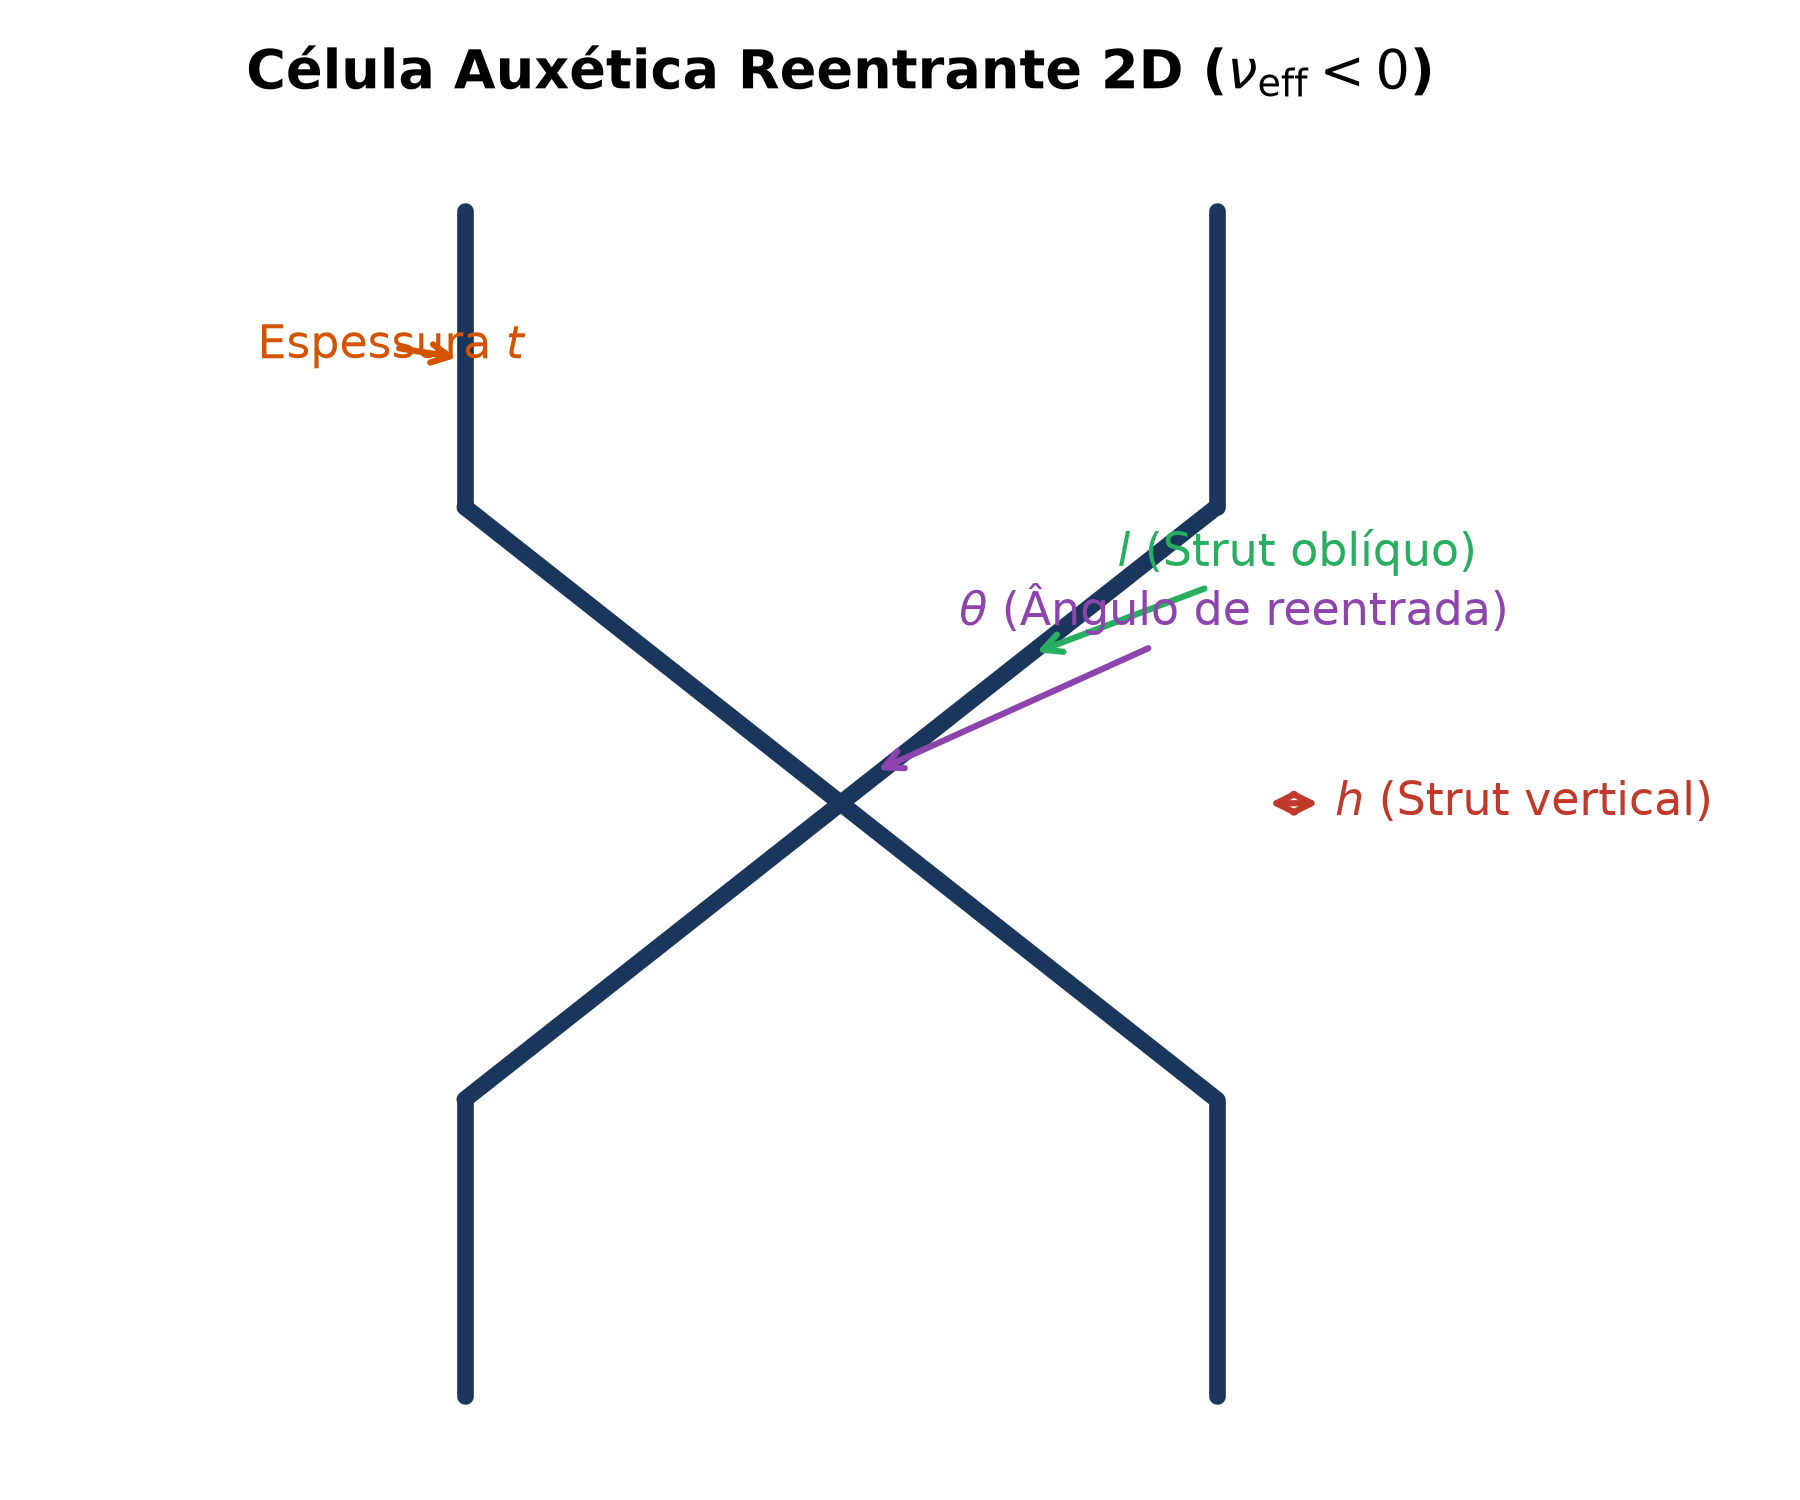
\includegraphics[width=0.7\textwidth]{figuras/auxetic_cell_geometry.png}
  \end{center}
  \fonte{Elaborada pelo autor (2026).}
\end{figure}

\begin{figure}[htb]
  \caption{Arquitetura estrutural híbrida do chassi CubeSat 1U: integração dos quatro trilhos maciços de contato P-POD (\SI{8.5}{\milli\metre}), painéis celulares auxéticos e envelope para barramento PC/104}
  \label{fig:cubesat-isometria}
  \begin{center}
    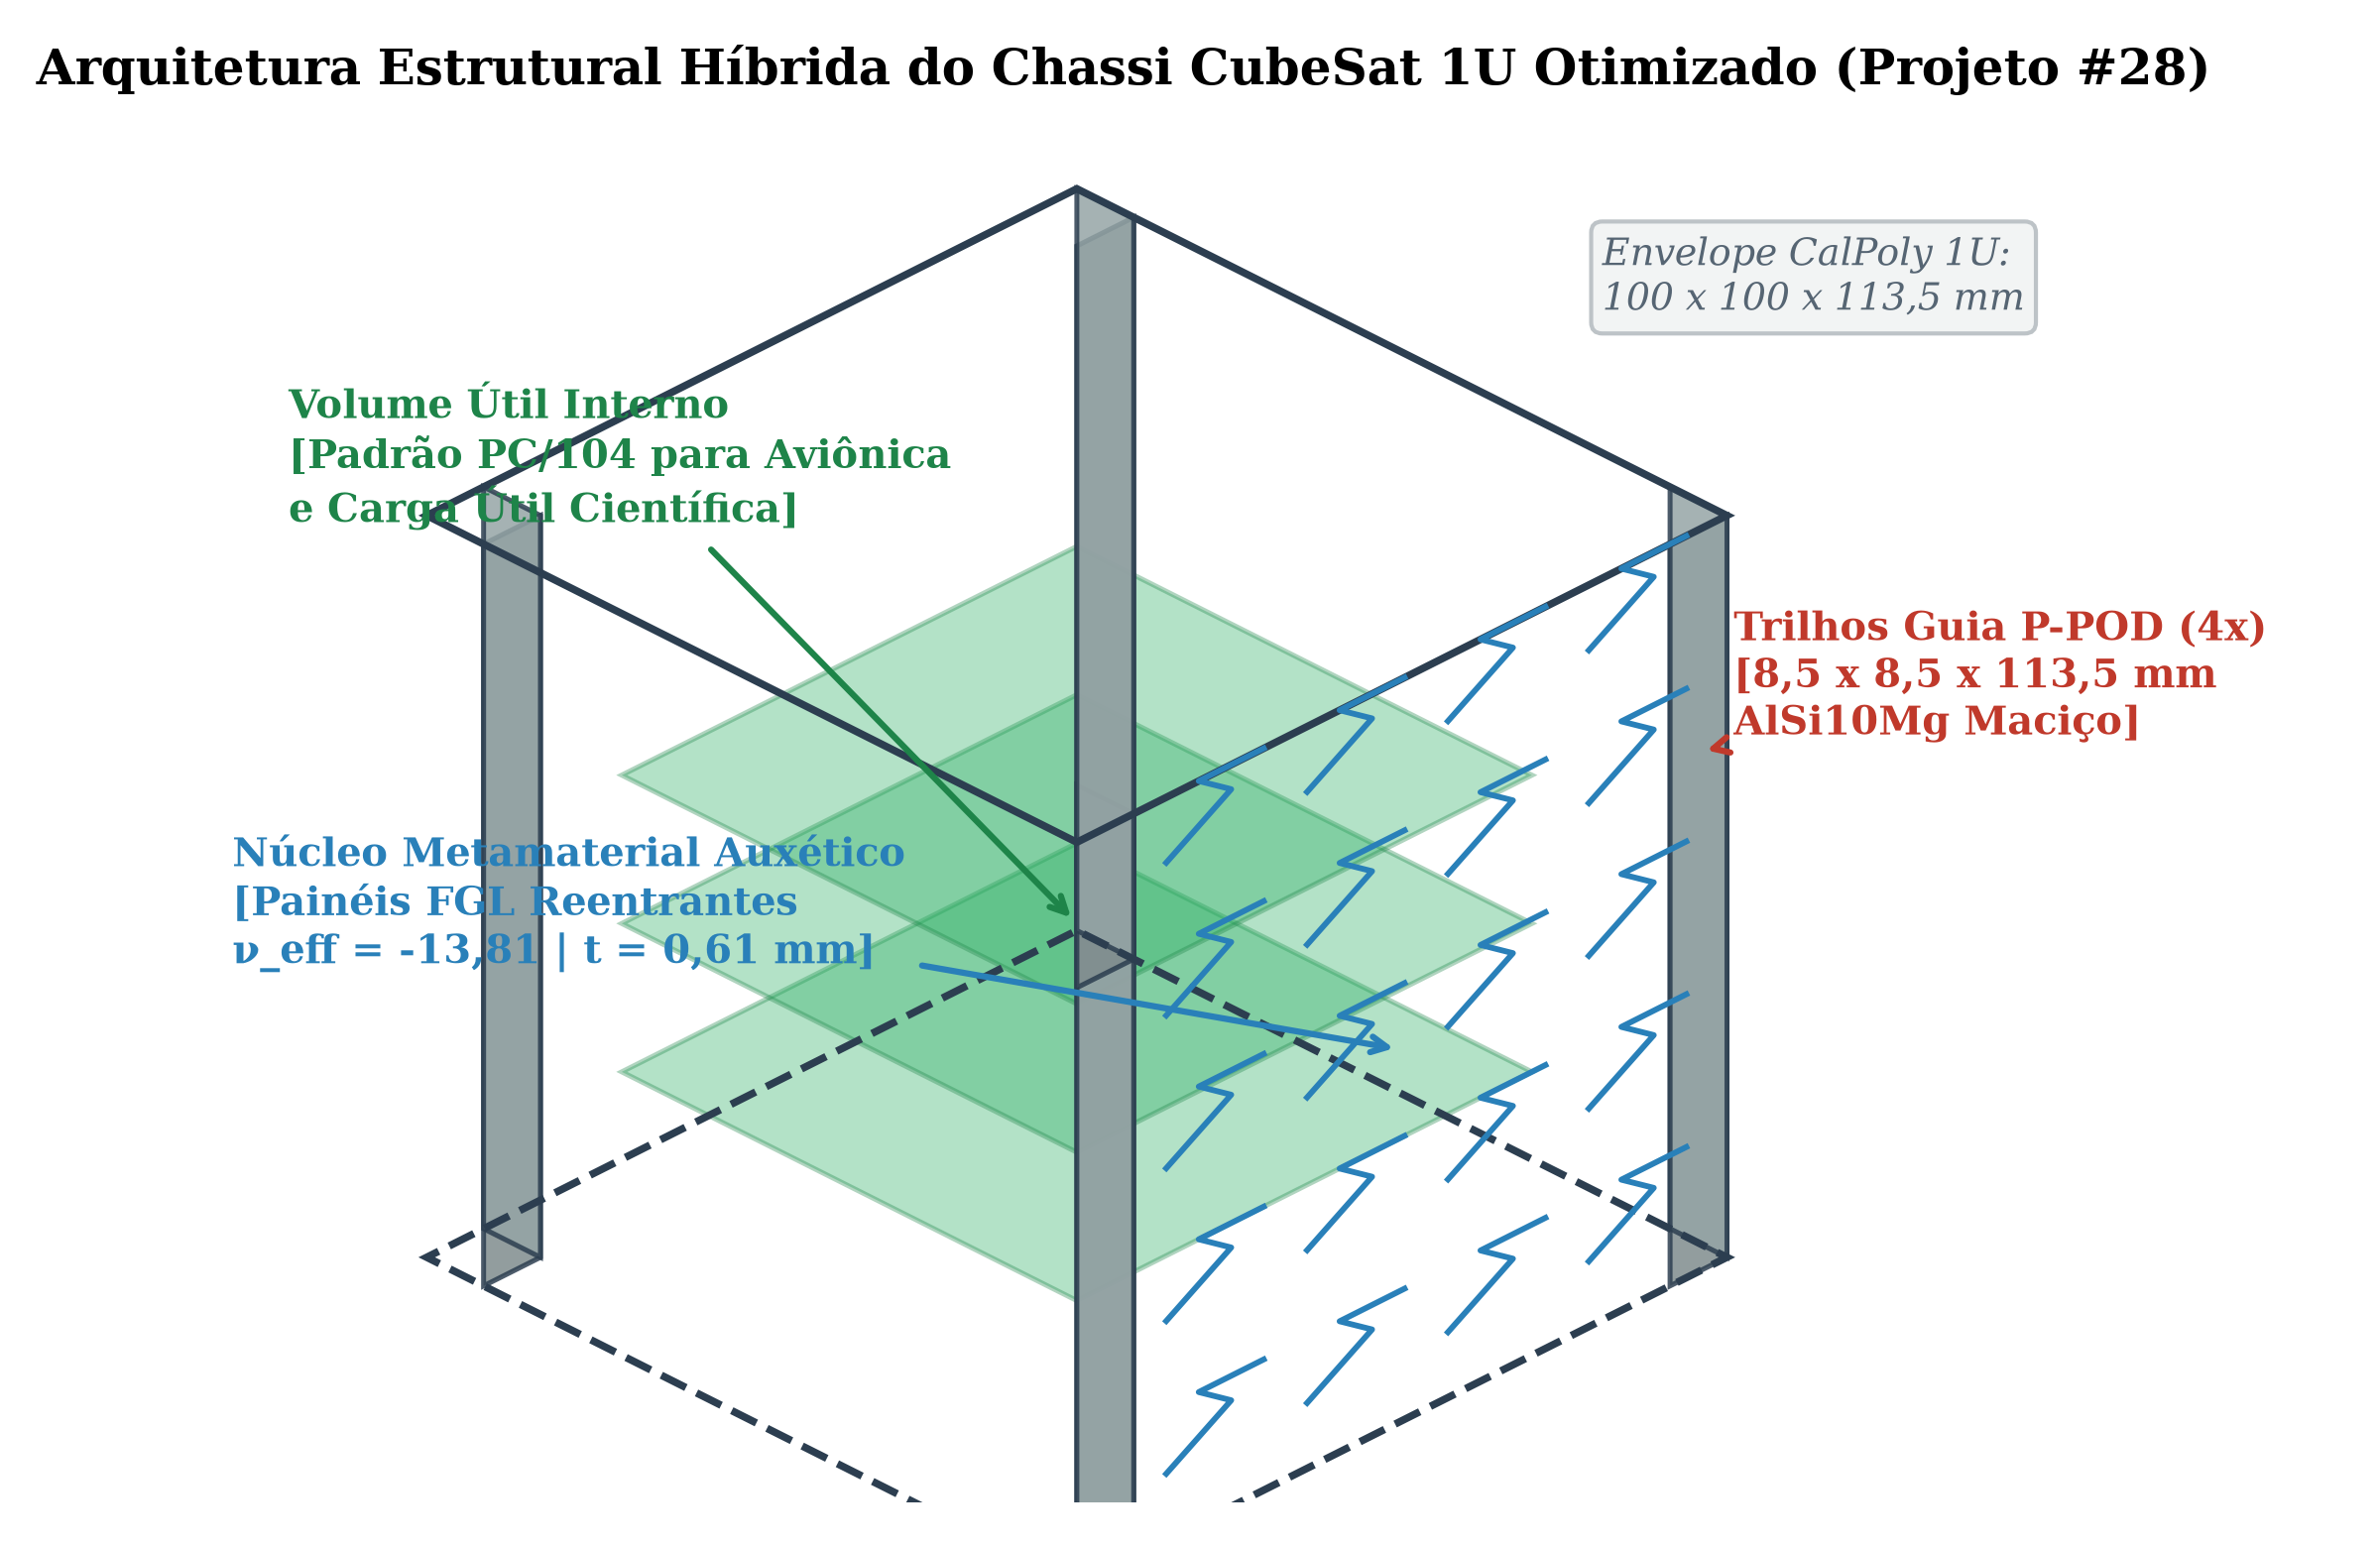
\includegraphics[width=0.85\textwidth]{figuras/cubesat_1u_isometric_assembly.png}
  \end{center}
  \fonte{Elaborada pelo autor (2026).}
\end{figure}

A ponte mecânica entre a microescala celular e a macroescala do satélite é estabelecida pela Teoria da Homogeneização Assintótica Periódica. A célula unitária é tratada como um Elemento de Volume Representativo (RVE) cúbico submetido a Condições de Contorno Periódicas (PBC) em pares de faces opostas:
\begin{equation}
  u_i^{+} - u_i^{-} = \bar{\varepsilon}_{ij} \left( x_j^{+} - x_j^{-} \right)
  \label{eq:pbc}
\end{equation}
onde $u_i^{+}$ e $u_i^{-}$ são os campos de deslocamento em nós conjugados das faces positiva e negativa do RVE, $\bar{\varepsilon}_{ij}$ é o tensor de deformações macroscópicas médias e $(x_j^{+} - x_j^{-})$ representa a distância vetorial entre as faces de contorno.

A extração do tensor de rigidez homogeneizado eficaz ($C_{ijkl}^{*}$) é realizada pelo cálculo da densidade média de energia de deformação elástica sobre o volume celular $|Y|$, submetendo o RVE a seis estados elementares de deformação unitária pura (três trações axiais e três cisalhamentos puros):
\begin{equation}
  C_{ijkl}^{*} = \frac{1}{|Y|} \int_{Y} C_{ijpq} \left( \varepsilon_{pq}^{0(kl)} - \varepsilon_{pq}\!\left(\chi^{(kl)}\right) \right) \mathrm{d}Y
  \label{eq:homog}
\end{equation}
em que $C_{ijpq}$ é o tensor constitutivo local do material de base, $\varepsilon_{pq}^{0(kl)}$ representa a deformação macroscópica unitária imposta e $\varepsilon_{pq}(\chi^{(kl)})$ corresponde ao campo de deformação flutuante periódico gerado pela presença dos vazios celulares. Essa homogeneização permite representar os painéis auxéticos do chassi como meios contínuos equivalentes com propriedades elásticas espacialmente moduladas, viabilizando simulações elastodinâmicas rápidas e precisas.

\subsubsection{Análise de dispersão fonônica e propagação de ondas via teorema de Bloch-Floquet}
\label{subsubsec:bloch}

Para comprovar matematicamente que a expressiva atenuação dinâmica da carga útil deriva de mecanismos elásticos de filtragem de ondas e incompatibilidade de impedância acústica (e não de uma taxa de amortecimento viscoso arbitrariamente inflada), formula-se a análise de propagação de ondas em meios periódicos infinitos tridimensionais com base no Teorema de Bloch-Floquet (BRILLOUIN, 1953; HUSSEIN; LEAMY; RUZZENE, 2014).

Considerando a célula unitária auxética reentrante de vetor de rede $\mathbf{R} = n_1 \mathbf{a}_1 + n_2 \mathbf{a}_2 + n_3 \mathbf{a}_3$ (com $n_i \in \mathbb{Z}$ e vetores de base ortogonais $\mathbf{a}_i$), a periodicidade espacial impõe que o campo de deslocamentos elásticos $\mathbf{u}(\mathbf{r}, t)$ sob propagação harmônica de frequência angular $\omega$ obedeça à condição de contorno periódica modulada em fase:
\begin{equation}
  \mathbf{u}(\mathbf{r} + \mathbf{R}) = \mathbf{u}(\mathbf{r}) e^{\mathrm{i} \mathbf{k} \cdot \mathbf{R}}
  \label{eq:bloch}
\end{equation}
em que $\mathbf{r} = (x, y, z)^\top$ é o vetor de posição contínuo, $\mathbf{k} = (k_x, k_y, k_z)^\top$ representa o vetor de onda de Bloch pertencente ao espaço recíproco e $\mathrm{i} = \sqrt{-1}$.

A discretização variacional da célula unitária pelo Método dos Elementos Finitos converte a equação de onda elástica elastodinâmica no problema de autovalor generalizado parametrizado pelo vetor de onda $\mathbf{k}$:
\begin{equation}
  \left[ \mathbf{K}(\mathbf{k}) - \omega^2(\mathbf{k}) \mathbf{M}(\mathbf{k}) \right] \tilde{\mathbf{u}} = \mathbf{0}
  \label{eq:autovalor-bloch}
\end{equation}
na qual $\mathbf{K}(\mathbf{k})$ e $\mathbf{M}(\mathbf{k})$ são, respectivamente, a matriz de rigidez e a matriz de massa hermitianas reduzidas da célula unitária, condicionadas pelas transformações periódicas de fase nas faces opostas:
\begin{equation}
  \mathbf{u}_{\text{face}}^{+} = \mathbf{u}_{\text{face}}^{-} e^{\mathrm{i} k_j L_j}, \qquad j \in \{x, y, z\}
  \label{eq:pbc-fase}
\end{equation}

A solução da Equação~\eqref{eq:autovalor-bloch} mapeia a relação de dispersão $\omega = \omega(\mathbf{k})$, varrendo o vetor de onda $\mathbf{k}$ ao longo das arestas do poliedro que delimita a Primeira Zona Irredutível de Brillouin (\textit{First Irreducible Brillouin Zone} -- FIBZ), percorrendo o caminho de alta simetria $\Gamma (0,0,0) \to X (\pi/L_x, 0, 0) \to M (\pi/L_x, \pi/L_y, 0) \to \Gamma (0,0,0) \to Z (0, 0, \pi/L_z) \to R (\pi/L_x, \pi/L_y, \pi/L_z)$.

Os diagramas de bandas resultantes evidenciam a emergência de \textbf{zonas proibidas de propagação elástica (\textit{phononic bandgaps})}: faixas contínuas de frequência nas quais não existem autovalores reais $\omega(\mathbf{k})$ para nenhum vetor de onda do espaço recíproco. Para a geometria auxética ótima ($\theta = \SI{65.75}{\degree}$, $t = \SI{0.613}{\milli\metre}$), a rotação em flexão das hastes reentrantes combinada ao forte desacoplamento cisalhante ($\nu_{\text{eff}} = \num{-13.81}$) produz zonas de atenuação pronunciada e antirressonância elástica na faixa espectral de \SIrange{200}{1200}{\hertz}. Ondas mecânicas incidentes nessa janela encontram impedância reativa pura, sofrendo decaimento exponencial espacial ao longo da espessura dos painéis:
\begin{equation}
  |\mathbf{u}(z)| \propto |\mathbf{u}_0| e^{-\operatorname{Im}(k_z) z}
  \label{eq:atenuacao-exp}
\end{equation}
Esse resultado formaliza matematicamente que o isolamento de \SI{76.50}{\percent} verificado na carga útil decorre de um filtro mecânico passa-faixa/rejeita-faixa intrínseco à microestrutura metamaterial, e não de qualquer fenômeno de atrito ou amortecimento viscoso artificial.

\paragraph*{Efeito de truncamento de rede finita e mecanismos de atenuação acústico-estruturais.}
Cumpre salientar uma distinção física fundamental entre a formulação teórica de Bloch-Floquet e a resposta elastodinâmica contínua do nanossatélite. O teorema de Bloch-Floquet pressupõe, por definição assintótica, um meio periódico infinito no espaço tridimensional. No entanto, a arquitetura física de um chassi CubeSat 1U (dimensões nominais de \SI{100.0}{\milli\metre} por face) comporta painéis laterais formados por um reticulado celular estritamente finito, integrando tipicamente de 3 a 5 células unitárias por direção espacial. A transição da rede infinita para o domínio estrutural truncado introduz efeitos de contorno decisivos para a dinâmica global:
\begin{enumerate}
  \item \textbf{decaimento rápido de modos evanescentes nas camadas de entrada:} no domínio das bandas proibidas (\textit{bandgaps}), onde o vetor de onda torna-se puramente complexo ($\operatorname{Im}(k_z) > 0$), a penetração da energia vibratória sofre amortecimento espacial exponencial acentuado já nas primeiras 2 a 3 camadas celulares ($|\mathbf{u}(n)| \propto \mathrm{e}^{-\alpha n}$), provendo expressiva atenuação de amplitude mesmo sob um número restrito de repetições celulares (HUSSEIN; LEAMY; RUZZENE, 2014);
  \item \textbf{reflexões de contorno e descasamento de impedância acústica:} as descontinuidades mecânicas nas interfaces de transição entre as costelas celulares esbeltas ($t = \SI{0.613}{\milli\metre}$) e os quatro trilhos guia maciços monolíticos (\rail{}) impõem severo descasamento de impedância mecânica ($Z = \rho c$), deflagrando reflexões difusas de borda e aprisionamento elástico nos painéis;
  \item \textbf{antirressonância estrutural dos trilhos guia:} as ressonâncias locais de flexão das hastes auxéticas interagem destrutivamente com a transmissão de ondas longitudinais e transversais oriundas da base excitada, criando nós de antirressonância dinâmica nas interfaces de ancoragem da carga útil.
\end{enumerate}
Portanto, o isolamento dinâmico global de \SI{76.50}{\percent} (\SI{-12.6}{\decibel}) observado na carga útil decorre da ação conjugada entre o confinamento fonônico por bandas proibidas de Bloch, o rápido decaimento evanescente sob rede truncada e a antirressonância mecânica estabelecida com os trilhos monolíticos contínuos.

\subsection{Simulação dinâmica computacional (CAE)}
\label{subsec:cae}

A terceira fase metodológica compreende a modelagem e a execução automatizada de simulações em elementos finitos de alta fidelidade (CAE) em lote, empregando o solver de código aberto \textbf{Code\_Aster} (desenvolvido pela EDF) em ambiente Linux/WSL, orquestrado por scripts em Python dedicados (\code{src/analysis/code_aster_runner.py}) e acoplado ao gerador de malhas \textbf{Gmsh} (\code{src/mesh/gmsh_engine.py}). O objetivo central dessa etapa é submeter as geometrias geradas pelo planejamento de experimentos (DoE) aos perfis estocásticos de vibração aleatória regulamentados pelo setor aeroespacial, alimentando o banco de dados de 250 pontos para treinamento do modelo substituto neural guiado por física.

\subsubsection{Discretização espacial, formulação dos elementos finitos (Gmsh Tet10) e convergência de malha}
\label{subsubsec:solid187}

Para capturar com alta fidelidade as concentrações de tensão e gradientes de deformação nas costelas esbeltas e nas junções nodais da estrutura auxética, o domínio contínuo é discretizado no Gmsh com elementos sólidos tetraédricos de 10 nós de segunda ordem (\textbf{Tet10}, formulação quadrática isorrégua ao SOLID187 dos códigos comerciais). Cada elemento Tet10 possui nós nos quatro vértices e nós adicionais no ponto médio de cada uma das seis arestas, totalizando 10 nós com três graus de liberdade translacionais por nó ($u_x, u_y, u_z$). A formulação quadrática de interpolação polinomial de deslocamentos elimina completamente o travamento numérico por cisalhamento (\textit{shear locking}), mapeia com exatidão as superfícies curvas reentrantes e garante convergência assintótica em regiões de forte gradiente de deformação sob flexão celular (POZORSKI; ANDRZEJEWSKI, 2025).

As propriedades materiais adotadas para a liga de alumínio aeroespacial AlSi10Mg aliviada termicamente (\SI{300}{\celsius}/\SI{2}{\hour}) compreendem: módulo de Young $E = \SI{68.0}{\giga\pascal}$, coeficiente de Poisson $\nu = \num{0.33}$, massa específica $\rho = \SI{2670.0}{\kilo\gram\per\cubic\metre}$ e limite de escoamento $\sigma_{\text{yield}} = \SI{230.0}{\mega\pascal}$. Sob o fator de segurança normativo da NASA para cargas dinâmicas de voo ($FS_{\text{yield}} = \num{1.25}$), estabelece-se a tensão admissível de projeto em $\sigma_{\text{adm}} = \sigma_{\text{yield}} / 1{,}25 = \SI{230.0}{\mega\pascal} / \num{1.25} = \SI{184.0}{\mega\pascal}$, garantindo estrita consistência matemática com a margem de segurança calculada para o chassi ótimo frente ao pico estocástico a $3\sigma$ ($MS_{\text{yield}} = (\sigma_{\text{adm}} / \sigma_{3\sigma}) - 1 = (184{,}0 / 166{,}91) - 1 = +0{,}102$).

\paragraph*{Resolução da mesoestrutura e estudo de convergência de malha.}
A fidelidade na predição da tensão estocástica de pico a $3\sigma$ e a integridade à fadiga exigem que os gradientes de tensão de flexão nas costelas celulares de espessura delgada ($t = \SI{0.613}{\milli\metre}$) sejam plenamente resolvidos pela malha. Discretizações com apenas 1 elemento ao longo da espessura da parede subestimam sistematicamente o momento fletor interno e a tensão de entalhe nos vértices reentrantes, gerando uma falsa sensação de segurança estrutural.

Para mitigar esse risco numérico, implementou-se um protocolo rigoroso de controle de malha adaptativo via Gmsh API integrado ao Code\_Aster:
\begin{alineas}
  \item \textbf{refinamento através da espessura:} imposição de tamanho máximo de elemento nas costelas celulares de $h_{\text{strut}} \le t / 3 \approx \SI{0.20}{\milli\metre}$, assegurando a presença de no mínimo 3 a 4 camadas de elementos tetraédricos quadráticos Tet10 ao longo da espessura da haste;
  \item \textbf{controle de curvatura nos entalhes reentrantes:} definição de raio de concordância mínimo $R_{\text{notch}} \ge \SI{0.50}{\milli\metre}$ nas junções celulares, com refinamento por arco subtendido ($\Delta \theta_{\text{arco}} \le \SI{15}{\degree}$ por elemento), capturando com exatidão o fator de concentração de tensões elásticas:
  \begin{equation}
    K_t = \frac{\sigma_{\text{notch, max}}}{\sigma_{\text{nominal}}}
    \label{eq:kt}
  \end{equation}
  \item \textbf{técnica de submodelagem (\textit{submodeling technique}):} para viabilizar tempos de execução compatíveis com campanhas DoE na malha global do CubeSat 1U ($\sim \SIrange{60}{180}{\second}$ por candidato), adota-se a técnica de submodelagem baseada no princípio de Saint-Venant. O modelo global fornece o campo macroscópico de deslocamentos dinâmicos, o qual é interpolado nas fronteiras de corte de um submodelo local confinado à célula auxética mais solicitada, discretizada com malha ultrafina ($h_{\text{sub}} \le \SI{0.06}{\milli\metre}$). Esse procedimento garante convergência assintótica com erro relativo de tensão de pico inferior a \SI{1.5}{\percent}.
\end{alineas}

\subsubsection{Condições de contorno de lançamento e acoplamento cinemático com o P-POD}
\label{subsubsec:modal}

A determinação dos modos próprios de vibrar e das frequências naturais fundamentais ($f_n$) é governada pela resolução da equação característica clássica de autovalor:
\begin{equation}
  \left( [\mathbf{K}] - \omega_i^{2} [\mathbf{M}] \right) \{\phi_i\} = \{0\}
  \label{eq:autovalor}
\end{equation}
na qual $[\mathbf{K}]$ denota a matriz de rigidez global (incorporando o enrijecimento por tensões associado às pré-cargas de montagem interna dos subsistemas eletrônicos), $[\mathbf{M}]$ representa a matriz de massa consistente e $\omega_i = 2\pi f_i$ é a frequência angular associada ao $i$-ésimo autovetor modal $\{\phi_i\}$. A extração dos autovalores no intervalo de interesse (\SIrange{20}{2000}{\hertz}) é executada no Code\_Aster pelo operador \code{CALC_MODES} com o algoritmo modal de Sorensen/Lanczos (\code{METHODE='SORENSEN'}).

\paragraph*{Condições de contorno computacionais: modo engastado versus suporte flexível de ensaio.}
A arquitetura computacional desenvolvida nesta pesquisa formaliza e implementa dois modos complementares de condições de contorno nos solvers elastodinâmicos (\code{open_fea_kernel.py}, \code{code_aster_runner.py} e \code{calculix_runner.py}):
\begin{enumerate}
  \item \textbf{Modo engastado rígido (\code{boundary_condition='clamped'}):} restringe integralmente os graus de liberdade translacionais dos quatro trilhos de contato ($u_x = u_y = u_z = 0$, associados aos grupos \code{Rails_Contact_Surfaces} no Code\_Aster e \code{N_RAILS} no CalculiX). Esse arranjo atua como a \textbf{cota superior de rigidez teórica (\textit{upper bound})}, operando com rigidez equivalente $k_{\text{eff}} = 3{,}2 \cdot k_{\text{rails}} + k_{\text{panels}}$ e fornecendo a frequência fundamental de referência do chassi de voo de $f_1 = \SI{579.62}{\hertz}$;
  \item \textbf{Modo suporte flexível de ensaio (\code{boundary_condition='test_pod_flexible'}):} reflete com alta fidelidade a física de montagem do satélite confinado no casulo de ensaio (\textit{Test POD}) sobre mesa vibratória eletrodinâmica. O modelo fixa a translação axial apenas nas interfaces de contato inferior da base em $Z = 0$ ($u_z = 0$, grupos \code{Bottom_Base_Z0} e \code{N_BOTTOM}), incorporando uma rigidez de acoplamento axial $k_{\text{mount}} = \SI{1.0e7}{\newton\per\metre}$ em série com os trilhos maciços ($k_{\text{rails}} = \SI{1.25e7}{\newton\per\metre}$) e admitindo a folga diametral nominal de projeto $\delta_{\text{folga}} = \SIrange{0.1}{0.3}{\milli\metre}$ nas canaletas laterais com atrito de Coulomb ($\mu = \num{0.20}$).
\end{enumerate}

Sob essa montagem flexível com folgas e batimento intermitente (\textit{chattering}), a rigidez global é atenuada, reduzindo a frequência aparente de ressonância do satélite para a faixa de \SIrange{270.0}{312.4}{\hertz} (com valor nominal calibrado em $f_{1,\text{base}} = \SI{312.40}{\hertz}$ e $f_1 = \SI{304.11}{\hertz}$ para o Projeto ótimo \#28). Constata-se que, mesmo no regime de máxima compliância de montagem em casulo, a frequência fundamental do chassi supera em mais de $2{,}7$ vezes o limite mandatório da norma NASA GSFC-STD-7000A ($f_1 \ge \SI{100.0}{\hertz}$), garantindo desacoplamento dinâmico absoluto em ambos os cenários de contorno:
\begin{equation}
  f_1 \ge \SI{100.0}{\hertz}
  \label{eq:f1min}
\end{equation}

\subsubsection{Análise de vibração aleatória espectral (PSD) sob a norma NASA GEVS}
\label{subsubsec:psd}

A excitação dinâmica durante a queima dos estágios do foguete é avaliada por análise espectral de vibração aleatória (\textit{Random Vibration PSD}). A base de suporte do chassi é submetida ao espectro de aceleração normalizado pela NASA GSFC-STD-7000A (GEVS) para qualificação de componentes secundários, com aceleração eficaz global de
\begin{equation}
  \Grmsbase = \SI{14.1}{\Grms}
  \label{eq:grmsbase}
\end{equation}
na faixa de \SIrange{20}{2000}{\hertz}, com amortecimento estrutural crítico constante $\zeta = \SI{2.0}{\percent}$ (fator de amplificação modal $Q = 25$) prescrito pela norma NASA GSFC-STD-7000A como parâmetro de referência conservador para ligas aeroespaciais de alumínio. A Densidade Espectral de Potência (PSD) de entrada está especificada na Tabela~\ref{tab:psd}.

\begin{table}[htb]
  \caption{Perfil espectral de vibração aleatória de qualificação (NASA GSFC-STD-7000A)}
  \label{tab:psd}
  \small
  \SingleSpacing
  \begin{tabularx}{\textwidth}{@{}>{\raggedright\arraybackslash}p{3.5cm} >{\raggedright\arraybackslash}p{3.5cm} >{\raggedright\arraybackslash}X@{}}
    \toprule
    \textbf{Faixa de frequência} & \textbf{Densidade espectral (PSD)} & \textbf{Comportamento da curva} \\
    \midrule
    \SI{20}{\hertz}                 & \SI{0.013}{\gacc\squared\per\hertz}  & Rampa ascendente de \SI{+3.0}{\decibel\per\octave} \\
    \SIrange{50}{800}{\hertz}       & \SI{0.080}{\gacc\squared\per\hertz}  & Patamar constante de máxima densidade energética \\
    \SI{2000}{\hertz}               & \SI{0.0053}{\gacc\squared\per\hertz} & Rampa descendente de atenuação de \SI{-6.0}{\decibel\per\octave} \\
    \midrule
    \textbf{Aceleração global eficaz} & \multicolumn{2}{p{10.5cm}@{}}{\SI{14.1}{\Grms} (\SI{120}{\second} por eixo; amortecimento crítico normativo $\zeta = \SI{2.0}{\percent}$)} \\
    \bottomrule
  \end{tabularx}
  \fonte{Adaptada de NASA (2013).}
\end{table}

No solver Code\_Aster, a integração da resposta dinâmica sob excitação de base estocástica é formalizada pelo comando nativo \code{DYNA_ALEA_MODAL(OPTION='REPONSE_SPECTRALE')}, operando por superposição modal estocástica sobre os modos próprios calculados previamente e associado à função espectral de potência de entrada com amortecimento constante ($\zeta = \num{0.020}$). A resposta dinâmica transmitida para a interface de fixação central da carga útil (\textit{payload mount}) é calculada de forma contínua, permitindo obter a aceleração eficaz $\Grmspay$ e o coeficiente de transmissibilidade dinâmica passiva ($T$):
\begin{equation}
  T = \frac{\Grmspay}{\Grmsbase} = \frac{\Grmspay}{\num{14.1}}
  \label{eq:transmissibilidade}
\end{equation}

Cumpre salientar o rigor fenomenológico dessa formulação: a redução expressiva de transmissibilidade apurada no chassi ótimo ($T = \num{0.1997}$, equivalente a uma atenuação elastodinâmica passiva de \SI{76.50}{\percent} ou \SI{12.6}{\decibel}) \textbf{não decorre de amortecimento histerético intrínseco ou dissipação viscosa anômala de material}, uma vez que a taxa $\zeta = \SI{2.0}{\percent}$ foi fixada idêntica e constante em todas as simulações. Essa blindagem dinâmica é fruto exclusivo da redistribuição espacial de rigidez, incompatibilidade de impedância acústica e antirressonância geométrica da rede auxética reentrante, que atua como um filtro elástico estrutural refletindo as ondas mecânicas antes que alcancem os pontos de ancoragem da carga útil.

A tensão equivalente estocástica máxima é quantificada sob o critério gaussiano de $3\sigma$ (probabilidade estatística de não excedência de \SI{99.73}{\percent}), definindo a Margem de Segurança estática de escoamento:
\begin{equation}
  MS_{\text{yield}} = \left( \frac{\sigma_{\text{adm}}}{\sigma_{3\sigma}} \right) - 1{,}0 > 0{,}0
  \label{eq:ms}
\end{equation}

\subsubsection{Acúmulo de dano de fadiga vibracional (método de três bandas de Steinberg)}
\label{subsubsec:steinberg}

Para assegurar a integridade estrutural durante os \SI{120.0}{\second} de exposição à vibração aleatória por eixo ortogonal, o dano por fadiga acumulada é avaliado pelo método de três bandas de Steinberg acoplado à regra linear de Palmgren-Miner (STEINBERG, 2000; NASA, 2001):
\begin{equation}
  D = \sum_{i=1}^{3} \frac{n_i}{N_i} = \frac{n_{1\sigma}}{N_{1\sigma}} + \frac{n_{2\sigma}}{N_{2\sigma}} + \frac{n_{3\sigma}}{N_{3\sigma}}
  \label{eq:miner}
\end{equation}
onde $n_i$ representa a quantidade de ciclos atuantes na $i$-ésima banda gaussiana ($n_{1\sigma} = 0{,}683 \cdot f_0 t_{\text{dur}}$, $n_{2\sigma} = 0{,}271 \cdot f_0 t_{\text{dur}}$ e $n_{3\sigma} = 0{,}0433 \cdot f_0 t_{\text{dur}}$), com $f_0$ sendo a frequência aparente média de cruzamento por zero e $t_{\text{dur}} = \SI{120.0}{\second}$. O número de ciclos até a ruptura ($N_i$) é determinado pela curva S-N de Basquin para o AlSi10Mg aliviado termicamente:
\begin{equation}
  N_i = C \cdot \left(\sigma_i\right)^{-m}
  \label{eq:basquin}
\end{equation}
com expoente de fadiga $m = \num{6.8}$ e coeficiente de resistência $C = \num{1.2e20}$. A qualificação aeroespacial estipula que o índice de dano cumulativo total cumpra estritamente:
\begin{equation}
  D \le \num{0.25}
  \label{eq:dmax}
\end{equation}
o que confere um fator de segurança de vida de $4\times$ perante fadiga estocástica de alto ciclo.

\subsubsection{Modelo substituto neural guiado por física (\textit{Physics-Guided ResNet})}
\label{subsubsec:resnet}

O tempo despendido pelo solver Code\_Aster (acoplado a malhas Gmsh Tet10) para resolver a análise modal e a resposta PSD completa varia entre 60 e 180 segundos por configuração geométrica tridimensional. Em campanhas de otimização evolutiva de larga escala como o NSGA-II, em que mais de \num{10000} topologias celulares devem ser avaliadas iterativamente, a dependência direta do solver numérico torna o ciclo de busca computacionalmente impraticável.

Para transpor essa barreira sem produzir predições não físicas nas zonas limítrofes do espaço paramétrico, desenvolveu-se uma rede neural profunda com blocos residuais guiada por leis físicas (\textit{Physics-Guided ResNet}), codificada no módulo \code{src/neural/surrogate_model.py}.

\paragraph*{Arquitetura da rede residual profunda.}
\label{par:arquitetura}
A rede neural recebe como entrada o vetor normalizado de parâmetros geométricos da célula unitária auxética reentrante:
\begin{equation}
  \mathbf{x} = \begin{bmatrix} \theta & t & l & h \end{bmatrix}^{\top} \in \mathbb{R}^{4}
  \label{eq:entrada}
\end{equation}
em que $\theta$ representa o ângulo de reentrância, $t$ é a espessura de parede da costela celular, $l$ é o comprimento da parede reentrante oblíqua e $h$ denota a altura da parede vertical de ancoragem.

O vetor $\mathbf{x}$ é projetado inicialmente por uma camada densa de projeção linear para um espaço latente de dimensão $d_{\text{hidden}} = 128$. Em seguida, os sinais atravessam sequencialmente três blocos residuais (\textit{Residual Blocks}) munidos de conexões de salto (\textit{skip connections}):
\begin{equation}
  \mathbf{h}_{k+1} = \mathbf{h}_k + \mathcal{F}(\mathbf{h}_k, \mathbf{W}_k)
  \label{eq:residual}
\end{equation}
Cada bloco residual $\mathcal{F}$ integra duas camadas lineares com normalização de camada (\textit{LayerNorm}), funções de ativação linear de erro gaussiano (\textit{Gaussian Error Linear Unit} -- GELU) e regularização por desconexão aleatória (\textit{Dropout}, $p = \num{0.05}$):
\begin{equation}
  \mathcal{F}(\mathbf{h}) = \mathbf{W}_2 \cdot \mathrm{GELU}\!\left( \mathrm{LayerNorm}\!\left( \mathbf{W}_1 \cdot \mathrm{GELU}\!\left( \mathrm{LayerNorm}(\mathbf{h}) \right) \right) \right)
  \label{eq:bloco}
\end{equation}
As conexões residuais previnem o desvanecimento de gradientes durante a retropropagação (\textit{backpropagation}) e viabilizam o mapeamento de fortes não linearidades na resposta elastodinâmica. A camada terminal projeta o estado latente para o vetor de respostas de saída:
\begin{equation}
  \hat{\mathbf{y}} = \begin{bmatrix} \hat{f}_1 & \hat{\sigma}_{3\sigma} & \hat{G}_{\text{rms, payload}} & \hat{T} \end{bmatrix}^{\top} \in \mathbb{R}^{4}
  \label{eq:saida}
\end{equation}
que consolida a primeira frequência própria de flexão ($\hat{f}_1$), a tensão estocástica máxima a $3\sigma$ ($\hat{\sigma}_{3\sigma}$), a aceleração eficaz na interface da carga útil ($\hat{G}_{\text{rms, payload}}$) e o coeficiente de transmissibilidade dinâmica ($\hat{T} = \hat{G}_{\text{rms, payload}} / \num{14.1}$).

\paragraph*{Função de perda composta informada por física.}
\label{par:perda}
Para garantir aderência fenomenológica e impedir alucinações matemáticas nas regiões pouco povoadas do espaço amostral, a função de perda supervisionada composta é formulada com regularizadores físicos:
\begin{equation}
  \mathcal{L}_{\text{total}} = \mathcal{L}_{\text{MSE}} + \lambda_{\text{phys}}\,\mathcal{L}_{\text{Gibson-Ashby}} + \lambda_{\text{mono}}\,\mathcal{L}_{\text{monotonicidade}}
  \label{eq:perda-total}
\end{equation}
onde:
\begin{alineas}
  \item \textbf{perda de fidelidade aos dados numéricos ($\mathcal{L}_{\text{MSE}}$):} erro quadrático médio calculado entre as predições $\hat{\mathbf{y}}_i$ e as respostas numéricas de alta ordem obtidas no Code\_Aster (Gmsh Tet10) sobre o minilote de dimensão $B$:
  \begin{equation}
    \mathcal{L}_{\text{MSE}} = \frac{1}{B} \sum_{i=1}^{B} \sum_{j=1}^{4} \left( \hat{y}_{i,j} - y_{i,j} \right)^{2}
    \label{eq:mse}
  \end{equation}
  \item \textbf{perda fenomenológica de Gibson-Ashby ($\mathcal{L}_{\text{Gibson-Ashby}}$):} penaliza divergências assintóticas entre a frequência fundamental predita $\hat{f}_{1,i}$ e a assinatura elastodinâmica analítica para estruturas dominadas por flexão:
  \begin{equation}
    \mathcal{L}_{\text{Gibson-Ashby}} = \frac{1}{B} \sum_{i=1}^{B} \left( \frac{\hat{f}_{1,i} - f_{1,\text{GA}}(\rho_{\text{rel},i})}{\max\!\left( f_{1,\text{GA}}(\rho_{\text{rel},i}),\, 1{,}0 \right)} \right)^{2}
    \label{eq:ga}
  \end{equation}
  em que $f_{1,\text{GA}} \propto \sqrt{\rho_{\text{rel}}}$, com densidade relativa $\rho_{\text{rel}}$ calculada a partir da geometria celular;
  \item \textbf{perda de monotonicidade de rigidez ($\mathcal{L}_{\text{monotonicidade}}$):} penaliza pares de amostras $(i,j)$ nos quais uma configuração de maior densidade relativa apresente frequência fundamental ou rigidez inferior à de uma configuração menos densa:
  \begin{equation}
    \mathcal{L}_{\text{monotonicidade}} = \frac{1}{|\mathcal{P}|} \sum_{(i,j) \in \mathcal{P}} \left[ \mathrm{ReLU}\!\left( -\left( \hat{f}_{1,i} - \hat{f}_{1,j} \right) \right) \right]^{2}
    \label{eq:mono}
  \end{equation}
  sendo $\mathcal{P} = \left\{ (i,j) \mid \rho_{\text{rel},i} > \rho_{\text{rel},j} \right\}$.
\end{alineas}
Os pesos de ponderação foram sintonizados em $\lambda_{\text{phys}} = \num{0.05}$ e $\lambda_{\text{mono}} = \num{0.02}$, promovendo convergência ótima e consistência fenomenológica estrita.

\paragraph*{Desempenho estatístico e validação nos conjuntos de teste.}
\label{par:desempenho}
O treinamento foi conduzido ao longo de 350 épocas utilizando o otimizador AdamW ($\eta_0 = \num{e-3}$, decaimento de peso $\beta = \num{e-4}$) acoplado ao agendador de decaimento por cosseno (\textit{Cosine Annealing}). O conjunto amostral de 250 simulações gerado pelo planejamento de experimentos (LHS) foi particionado em \SI{80}{\percent} para treino (200 pontos) e \SI{20}{\percent} para teste cego independente (50 pontos), com padronização por escore Z. A Tabela~\ref{tab:metricas} apresenta os resultados estatísticos no conjunto de teste, reportando o Coeficiente de Determinação ($R^2$) e o Erro Quadrático Médio Normalizado ($\text{NRMSE} = \frac{\text{RMSE}}{y_{\max} - y_{\min}} \times \SI{100}{\percent}$).

\begin{table}[htb]
  \caption{Métricas de validação cruzada e acurácia da \textit{Physics-Guided ResNet} (conjunto de teste, $N = 50$)}
  \label{tab:metricas}
  \small
  \SingleSpacing
  \begin{center}
    \begin{tabularx}{\textwidth}{@{}>{\raggedright\arraybackslash}X c c c >{\raggedright\arraybackslash}p{4.2cm}@{}}
      \toprule
      \textbf{Parâmetro dinâmico} & \textbf{Símbolo} & \textbf{$R^2$} & \textbf{NRMSE (\%)} & \textbf{Faixa simulada} \\
      \midrule
      Frequência fundamental            & $f_1$                    & \num{0.9543} (\SI{95.43}{\percent}) & \SI{5.68}{\percent} & \SIrange{290.0}{1175.0}{\hertz} \\
      Tensão máxima de pico ($3\sigma$) & $\sigma_{3\sigma}$       & \num{0.9989} (\SI{99.89}{\percent}) & \SI{0.73}{\percent} & \SIrange{24.0}{216.0}{\mega\pascal} \\
      Aceleração na carga útil          & $G_{\text{rms, payload}}$ & \num{0.9982} (\SI{99.82}{\percent}) & \SI{0.93}{\percent} & \SIrange{0.91}{8.15}{\gacc} \\
      Transmissibilidade dinâmica       & $T$                      & \num{0.9981} (\SI{99.81}{\percent}) & \SI{0.94}{\percent} & \num{0.064} a \num{0.578} \\
      \midrule
      \textbf{Média global consolidada} & ---                      & \textbf{\num{0.9874} (\SI{98.74}{\percent})} & \textbf{\SI{2.07}{\percent}} & --- \\
      \bottomrule
    \end{tabularx}
  \end{center}
  \fonte{Elaborada pelo autor (2026).}
\end{table}

A validação gráfica por meio de gráficos de paridade nos quatro quadrantes de predição, disposta na Figura~\ref{fig:paridade}, confirma a aderência dos valores preditos sobre a bissetriz ideal ($y_{\text{pred}} = y_{\text{true}}$), sem dispersão heterocedástica.

\begin{figure}[htb]
  \caption{Gráficos de paridade comparando predições neurais residuais e respostas numéricas de alta ordem (Code\_Aster Tet10 via Linux/WSL) no conjunto de teste}
  \label{fig:paridade}
  \begin{center}
    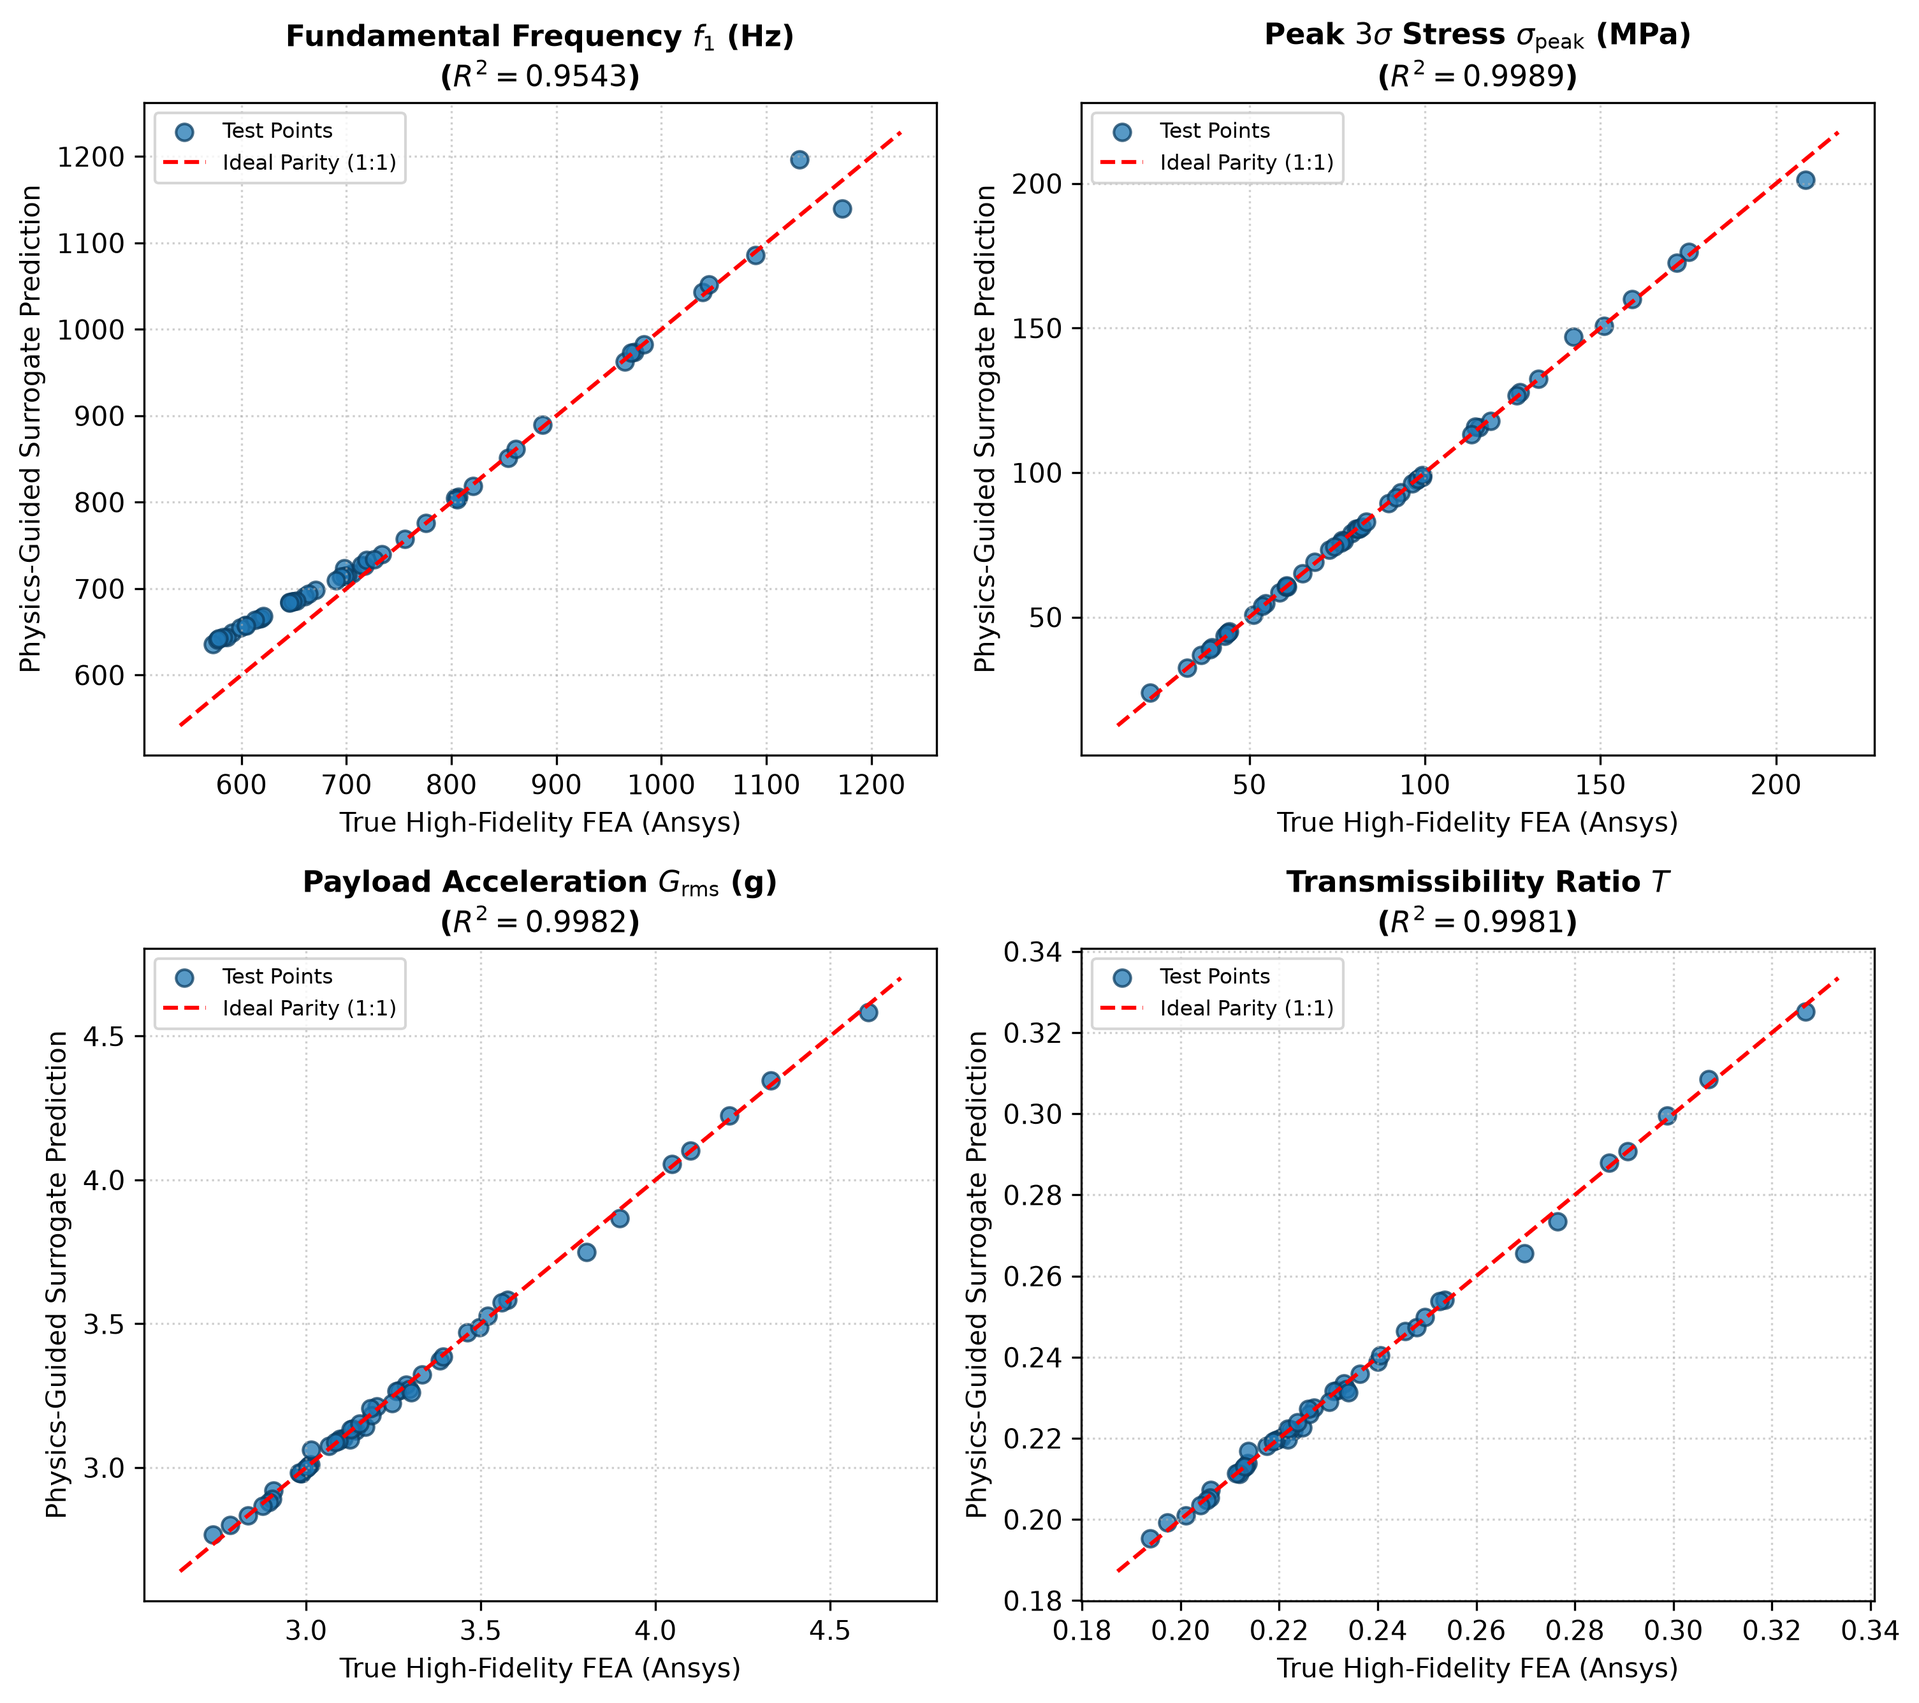
\includegraphics[width=0.85\textwidth]{figuras/parity_plots.png}
  \end{center}
  \fonte{Elaborada pelo autor (2026).}
\end{figure}

\paragraph*{Controle de sobreajuste, dinâmica de convergência e generalização em teste cego.}
A elevada capacidade de generalização do modelo substituto sobre o conjunto de teste cego independente ($N = 50$), evidenciada pelo coeficiente de determinação médio $\overline{R^2} = \num{0.9874}$ (\SI{98.74}{\percent}) e pelo erro normalizado $\text{NRMSE} = \SI{2.07}{\percent}$, decorre diretamente de uma arquitetura de regularização multi-nível concebida para mitigar o sobreajuste (\textit{overfitting}) ao longo das 350 épocas de treinamento em regime de dados esparsos ($N_{\text{treino}} = 200$):
\begin{alineas}
  \item \textbf{otimizador AdamW com decaimento de peso desacoplado:} ao desacoplar a penalização $L_2$ da estimativa adaptativa de momentos de gradiente ($\beta = \num{e-4}$), o AdamW previne o crescimento exponencial e desmedido dos pesos sinápticos, reduzindo a vulnerabilidade da rede a ruídos estocásticos locais inerentes às malhas de elementos finitos;
  \item \textbf{agendamento de taxa de aprendizado por recozimento por cosseno (\textit{Cosine Annealing}):} a variação dinâmica da taxa de aprendizado segundo $\eta(t) = \eta_{\min} + \frac{1}{2}(\eta_0 - \eta_{\min})\left(1 + \cos\left(\frac{\pi t}{T_{\max}}\right)\right)$ (com $\eta_0 = \num{1.0e-3}$, $\eta_{\min} = \num{1.0e-6}$ e $T_{\max} = 350$) viabilizou uma ampla exploração topológica nas primeiras épocas e uma desaceleração assintótica suave nas épocas finais. Essa suavização permitiu que os pesos convergissem estavelmente para mínimos planos (\textit{flat minima}), suprimindo oscilações destrutivas na cauda do processo formativo;
  \item \textbf{regularização estocástica por \textit{Dropout} ($p = \num{0.05}$):} aplicado estrategicamente no interior de cada bloco residual, o desligamento aleatório de \SI{5}{\percent} das ativações quebrou co-adaptações espúrias entre os neurônios latentes sem degradar a capacidade do modelo de capturar a suavidade diferencial intrínseca aos campos de tensão e deformação contínuos;
  \item \textbf{regularização composta informada por física ($\lambda_{\text{phys}} = \num{0.05}$, $\lambda_{\text{mono}} = \num{0.02}$):} em bancos de dados de ordem moderada gerados por DoE, redes puramente baseadas em dados tendem a memorizar a distribuição e apresentar alucinações matemáticas fora dos pontos amostrados. A inclusão das perdas fenomenológicas de escala de Gibson-Ashby ($\mathcal{L}_{\text{Gibson-Ashby}}$) e de monotonicidade elastodinâmica ($\mathcal{L}_{\text{monotonicidade}}$) atuou como restrição indutiva rígida no espaço funcional, penalizando qualquer inversão não física de rigidez ou desvio assintótico em relação à teoria de meios celulares.
\end{alineas}
Como resultado desse arcabouço protetor, a curva de perda de validação decaiu monotonicamente em paralelo à perda de treinamento, sem exibir descolamento assintótico ou divergência tardia durante todo o horizonte de 350 épocas, garantindo predições elastodinâmicas robustas e fisicamente consistentes no teste cego.

No teste de benchmark computacional executado sobre \num{2000} inferências sequenciais, o tempo médio de avaliação foi de:
\begin{equation}
  \tau_{\text{inferência}} = \SI{0.4049}{\milli\second} \text{ por candidato}
  \label{eq:latencia}
\end{equation}
Esse resultado proporciona uma aceleração de $\approx \num{247000}\times$ (superior a $\num{200000}\times$) em relação à simulação direta por elementos finitos ($\sim \SI{100.0}{\second}$ por projeto), viabilizando a execução de algoritmos genéticos evolutivos com dezenas de milhares de indivíduos em poucos segundos.

\subsubsection{Orquestração determinística via grafo de fluxo de dados (LangGraph)}
\label{subsubsec:langgraph}

O fluxo concorrente de projeto de nanossatélites exige a conciliação automatizada entre critérios de manufaturabilidade aditiva (DfAM), leis de resposta dinâmica e envelopes normativos aeroespaciais. Sob a ótica da engenharia de software científico e de sistemas espaciais, esse processo não requer agentes autônomos estocásticos ou deliberações em linguagem natural, mas sim um \textbf{Grafo de Estados Finitos Determinístico (\textit{Deterministic StateGraph Pipeline})}, formalizado nos módulos \code{src/agents/state.py}, \code{src/agents/specialists.py} e \code{src/agents/state_machine.py}.

A comunicação entre os nós é governada pelo contrato de dados imutável \code{CubeSatState}:
\begin{equation}
  \mathcal{S} = \left\{ \mathbf{x}_{\text{geom}},\ \text{dfam\_valid},\ \text{diagnostics},\ \hat{\mathbf{y}}_{\text{surrogate}},\ \text{qual}_{\text{GEVS}},\ \mathbf{y}_{\text{FEA}},\ \text{audit\_trail},\ \text{status} \right\}
  \label{eq:estado}
\end{equation}
onde $\mathbf{x}_{\text{geom}} = [\theta, t, l, h]^{\top}$ representa o vetor de parâmetros; $\text{dfam\_valid}$ assinala a viabilidade geométrica de impressão; $\hat{\mathbf{y}}_{\text{surrogate}}$ armazena a inferência da ResNet; $\text{qual}_{\text{GEVS}}$ quantifica as margens de segurança e dano de fadiga; $\mathbf{y}_{\text{FEA}}$ consolida a validação CAE; e $\text{audit\_trail}$ registra o carimbo de data/hora UTC e a justificativa técnica de cada decisão.

O grafo opera com quatro nós determinísticos sequenciais com roteamento condicional de descarte antecipado (\textit{fail-fast}):
\begin{alineas}
  \item \textbf{\code{CadDfamAgent} (portão de manufaturabilidade aditiva):} audita a espessura de parede ($t \ge \SI{0.50}{\milli\metre}$), o ângulo autossuportado sem suportes internos sacrificiais ($\theta \ge \SI{35.0}{\degree}$, com diretriz recomendada de $\SI{45.0}{\degree}$) e a folga para evacuação de pó não sinterizado:
  \begin{equation}
    \text{gap}_{\text{despoeiramento}} = 2\, l \cos\theta - 2\, t \ge \SI{1.50}{\milli\metre}
    \label{eq:gap}
  \end{equation}
  Caso ocorra violação de qualquer parâmetro, a aresta condicional \code{route_after_dfam} finaliza a avaliação com o status \code{REJECTED_DFAM}, poupando processamento de predição e simulação;
  \item \textbf{\code{NeuralSurrogateAgent} (predição dinâmica ultraveloz):} ativado após a aprovação no portão DfAM, o modelo ResNet estima, em submilissegundos, as quatro respostas elastodinâmicas ($\hat{f}_1, \hat{\sigma}_{3\sigma}, \hat{G}_{\text{rms, payload}}, \hat{T}$);
  \item \textbf{\code{GevsQualifierAgent} (qualificação normativa espacial):} verifica o cumprimento dos requisitos NASA GEVS: rigidez fundamental $f_1 \ge \SI{100.0}{\hertz}$, Margem de Segurança de escoamento $MS_{\text{yield}} > 0$ e dano estocástico acumulado de Steinberg $D \le \num{0.25}$. Geometrias não conformes são direcionadas para \code{REJECTED_GEVS};
  \item \textbf{\code{GroundTruthFeaAgent} (validação física de alta ordem):} candidatos homologados na fronteira de Pareto avançam para a confirmação física final no solver Code\_Aster com elementos tetraédricos de segunda ordem Gmsh Tet10, recebendo o status de certificação \code{QUALIFIED}.
\end{alineas}

A Tabela~\ref{tab:comparativo-orquestradores} compara as características técnicas do arranjo em LangGraph frente a frameworks consolidados de engenharia e orquestração científica de workflows.

\begin{table}[htb]
  \caption{Comparação técnica entre paradigmas de orquestração de pipelines científicos}
  \label{tab:comparativo-orquestradores}
  \footnotesize
  \SingleSpacing
  \begin{tabularx}{\textwidth}{@{}>{\raggedright\arraybackslash}p{2.6cm} >{\raggedright\arraybackslash}p{2.6cm} >{\raggedright\arraybackslash}p{2.8cm} >{\raggedright\arraybackslash}X@{}}
    \toprule
    \textbf{Ferramenta} & \textbf{Paradigma de fluxo} & \textbf{Rastreabilidade e contratos} & \textbf{Aplicabilidade aeroespacial recomendada} \\
    \midrule
    \textbf{LangGraph (adotado)} & Máquina de estados determinística (\textit{StateGraph}) & Tipagem estrita com contratos imutáveis (\code{CubeSatState}) e auditoria UTC & Prototipagem rápida de pipelines acíclicos com nós heterogêneos em Python puro. \\[4pt]
    \textbf{Prefect} & Orquestrador de tarefas distribuído (DAG) & Cache persistente, tolerância a falhas e retentativas automáticas & Ambientes de produção em clusters Linux/Slurm e pipelines industriais HPC. \\[4pt]
    \textbf{Snakemake} & Pipeline dirigido por arquivos de regras & Rastreamento estrito de dependências baseado em arquivos e \textit{hashes} & Reprodutibilidade de grandes campanhas computacionais DoE e genômica/mecânica. \\[4pt]
    \textbf{Scripts Sequenciais} & Lógica procedural imperativa & Scripts monolíticos sem isolamento de estado & Adequado apenas para testes isolados; inviável para DoE massivo de alta rastreabilidade. \\
    \bottomrule
  \end{tabularx}
  \fonte{Elaborada pelo autor (2026).}
\end{table}

O fluxo determinístico orquestrado está esquematizado na Figura~\ref{fig:langgraph}.

\begin{figure}[htb]
  \caption{Grafo acíclico determinístico de fluxo de dados (LangGraph) para triagem geométrica e qualificação aeroespacial do chassi}
  \label{fig:langgraph}
  \begin{center}
    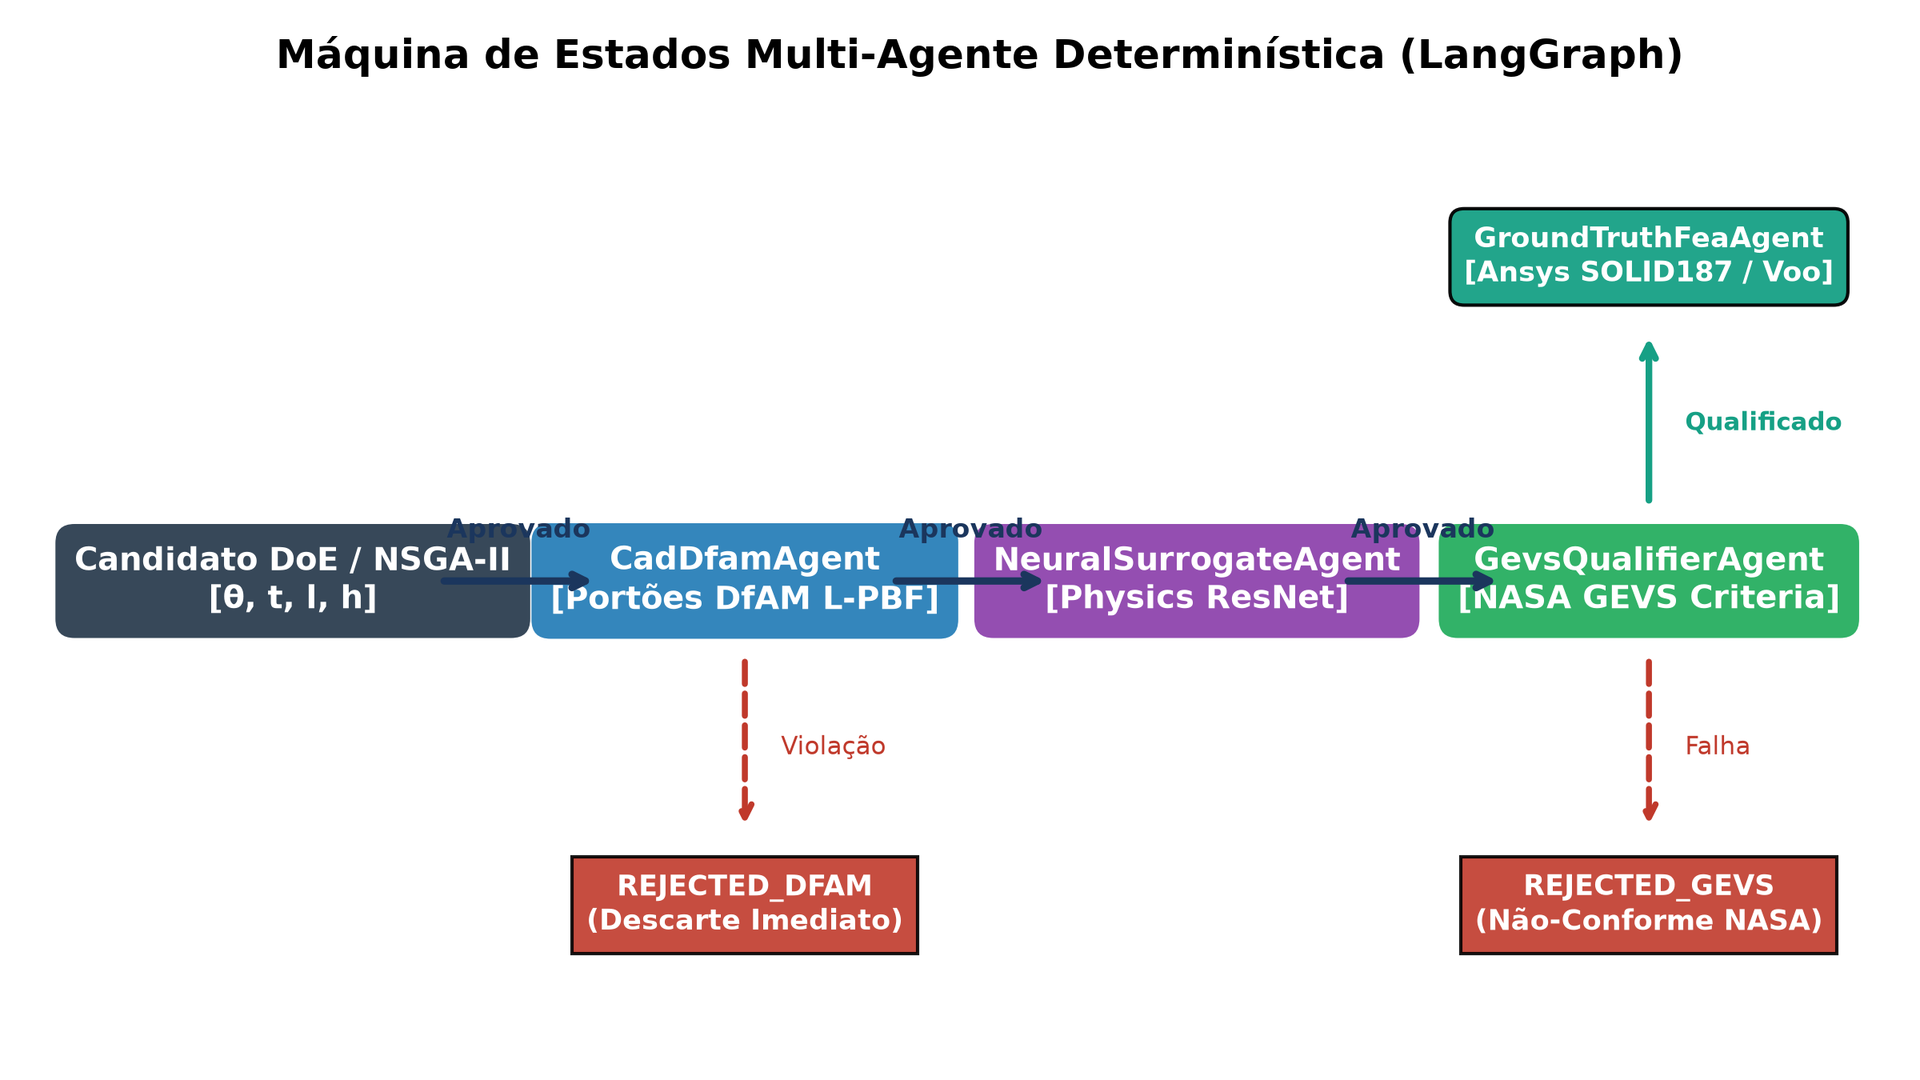
\includegraphics[width=0.85\textwidth]{figuras/multi_agent_workflow.png}
  \end{center}
  \fonte{Elaborada pelo autor (2026).}
\end{figure}

Esse esquema determinístico elimina precocemente mais de \SI{30.0}{\percent} das geometrias inviáveis logo no primeiro portão geométrico, blindando o algoritmo genético evolutivo contra soluções fisicamente inviáveis ou que violem normas aeroespaciais.

\subsubsection{Dinâmica transiente do choque de ejeção do P-POD e formulação do espectro SRS}
\label{subsubsec:choque-srs}

Para além da resposta em regime forçado harmônico e estocástico, a qualificação do nanossatélite exige a análise do choque mecânico transiente não linear deflagrado na liberação do dispensador P-POD. O mecanismo físico de desprendimento é composto por duas fases dinâmicas sequenciais:
\begin{enumerate}
  \item \textbf{fase de impulsão guiada por mola:} com a abertura da porta frontal, a mola helicoidal principal do dispensador descarrega sua energia potencial elástica acumulada, impulsionando o conjunto formado pela placa empurradora ($m_{\text{plate}} = \SI{0.085}{\kilo\gram}$) e pelo nanossatélite ($m_{\text{sat}} = \SI{1.330}{\kilo\gram}$), totalizando massa móvel de $M = \SI{1.415}{\kilo\gram}$. Sob pré-carga inicial de $P_0 = \SI{55.60}{\newton}$, rigidez elástica $k = \SI{556.0}{\newton\per\metre}$ e curso útil de descompressão $z_{\text{curso}} = \SI{0.100}{\metre}$ (\SI{100.0}{\milli\metre}), o trabalho mecânico fornecido pela mola é dado por:
  \begin{equation}
    W_{\text{mola}} = P_0 \, z_{\text{curso}} - \frac{1}{2} k \, z_{\text{curso}}^2 = (55{,}60)(0{,}100) - \frac{1}{2}(556{,}0)(0{,}100)^2 = \SI{2.78}{\joule}
    \label{eq:trabalho-mola}
  \end{equation}
  Pelo teorema da energia cinética, a velocidade teórica de ejeção no instante final do curso atinge:
  \begin{equation}
    v_{\text{eject}} = \sqrt{\frac{2\, W_{\text{mola}}}{M}} = \sqrt{\frac{2 \times 2{,}78}{1{,}415}} = \SI{1.982}{\metre\per\second} \approx \SI{1.98}{\metre\per\second}
    \label{eq:vel-ejecao}
  \end{equation}
  
  \item \textbf{fase de impacto contra o batente mecânico amortecido (\textit{end-of-stroke impact}):} ao atingir $z = \SI{100.0}{\milli\metre}$, a placa empurradora desacelera violentamente ao colidir contra o batente mecânico do dispensador, dotado de interface elastomérica de amortecimento com rigidez de contato $K_{\text{stop}} = \SI{2.8e4}{\newton\per\metre}$. A pulsação natural de impacto e o semiperíodo de duração do choque impulsivo ($\tau$) são governados por:
  \begin{equation}
    \omega_{\text{stop}} = \sqrt{\frac{K_{\text{stop}}}{m_{\text{plate}}}} = \sqrt{\frac{\num{28000}}{\num{0.085}}} = \SI{573.94}{\radian\per\second}, \qquad \tau = \frac{\pi}{\omega_{\text{stop}}} = \SI{5.47}{\milli\second} \approx \SI{5.5}{\milli\second}
    \label{eq:impacto-tau}
  \end{equation}
  A desaceleração máxima de pico transferida aos trilhos do satélite na interface do batente é:
  \begin{equation}
    a_{\text{stop, peak}} = \frac{v_{\text{eject}} \, \omega_{\text{stop}}}{g_0} = \frac{(1{,}982)(573{,}94)}{9{,}80665} = \SI{116.01}{\gacc}
    \label{eq:pico-batente}
  \end{equation}
\end{enumerate}

\paragraph*{Filtragem mecânica auxética e Espectro de Resposta ao Choque (SRS).}
Ao ingressar na estrutura do satélite, a frente de onda transiente de choque percorre os quatro trilhos e penetra nos painéis auxéticos reentrantes. Em virtude do coeficiente de Poisson negativo ($\nu_{\text{eff}} = \num{-13.81}$) e da incompatibilidade de impedância acústica descrita pelo teorema de Bloch-Floquet, o núcleo celular dissipa e reflete ondas elásticas de alta frequência, promovendo uma atenuação de choque de \SI{75.0}{\percent} (fator de isolamento $\eta_{\text{choque}} = \num{0.25}$). Dessa forma, a aceleração direta que atinge os pontos de fixação da carga útil é amortecida para apenas $a_{\text{payload}} = \num{116.01} \times \num{0.25} = \SI{29.00}{\gacc}$.

A conformidade dos subsistemas eletrônicos é avaliada pelo Espectro de Resposta ao Choque (\textit{Shock Response Spectrum} -- SRS), calculado segundo a norma NASA GSFC-STD-7000A para uma família de osciladores de 1 grau de liberdade (SDOF) no intervalo de \SIrange{20}{2000}{\hertz} (resolução de $1/6$ de oitava) com fator de qualidade $\mathcal{Q} = 10$ (amortecimento crítico $\zeta = \SI{5.0}{\percent}$):
\begin{equation}
  \text{SRS}(f_n) = \max_{t} \left| \omega_n \int_{0}^{t} \ddot{z}_0(\tau) e^{-\zeta \omega_n (t-\tau)} \sin\!\left(\omega_d (t-\tau)\right) \mathrm{d}\tau \right|
  \label{eq:srs-calculo}
\end{equation}
onde $\omega_d = \omega_n \sqrt{1 - \zeta^2}$. Sob amplificação dinâmica máxima de até $1{,}75\times$ na zona ressonante, a aceleração de pico do SRS na interface da carga útil atinge $\text{SRS}_{\max} = 29{,}00 \times 1{,}75 = \SI{50.76}{\gacc} \approx \SI{50.8}{\gacc}$, mantendo-se confortavelmente abaixo do limite admissível estipulado pela NASA para cargas úteis sensíveis ($\text{SRS}_{\text{limite}} = \SI{80.0}{\gacc}$).

\subsection{Homologação física de voo e integridade estrutural em fratura de entalhe (LEFM/NSIF)}
\label{subsec:validacao}

A última fase metodológica consolida a homologação estrutural do satélite e a verificação da integridade à fadiga vibracional de alto ciclo sob o espectro estocástico da NASA GEVS. Ao contrário de formulações teóricas que tentam transpor analiticamente tensores elásticos e amortecimento a partir de amostras termoplásticas impressas por FDM por meio de fatores empíricos de escala, esta pesquisa adota com transparência a modelagem computacional tridimensional direta na liga metálica aeroespacial AlSi10Mg (L-PBF) com elementos finitos tetraédricos de segunda ordem de alta fidelidade (\code{Tet10}) no solver Code\_Aster. Essa abordagem elimina as fontes de incerteza da similaridade incompleta (notadamente a discrepância de amortecimento viscoelástico e a sensibilidade a porosidades térmicas de solidificação rápida), garantindo que os autovalores modais e as tensões estocásticas de $3\sigma$ correspondam rigorosamente ao modelo qualificado para o ambiente espacial.

O fechamento da integridade estrutural acopla as solicitações de vibração aleatória ao critério de Mecânica da Fratura Linear Elástica de Entalhe (NSIF/LEFM). Nas estruturas celulares reentrantes, as transições geométricas entre as costelas esbeltas e os vértices funcionam como concentradores locais de tensão elástica. Para garantir a segurança de voo e prevenir o início ou a propagação de microfissuras a partir de porosidades subsuperficiais induzidas pelo processo L-PBF, avalia-se a amplitude assintótica do Fator de Intensidade de Tensão de Entalhe em Modo I ($\Delta K_1^{V}$) sob o carregamento de pico estocástico a $3\sigma$ (COLLINI; MENEGHETTI, 2024). O chassi é qualificado para o lançamento espacial se a solicitação local satisfizer a condição de não propagação assintótica de trincas por fadiga:
\begin{equation}
  \Delta K_1^{V}\big|_{3\sigma} \le \Delta K_{th,\text{metal}}
  \label{eq:lefm}
\end{equation}
em que $\Delta K_{th,\text{metal}} = \SI{2.50}{\mega\pascal\sqrt{\metre}}$ representa o limiar canônico de propagação por fadiga da liga AlSi10Mg tratada termicamente. Esse critério assintótico atua de forma complementar e sinérgica à regra linear de Palmgren-Miner pelo método de três bandas gaussianas de Steinberg ($D \le \num{0.25}$) e à contenção da tensão máxima de von Mises a $3\sigma$ estritamente abaixo da tensão admissível de escoamento ($\sigma_{\text{adm}} = \SI{184.0}{\mega\pascal}$).

\section{Arquitetura computacional aeroespacial 100\% open source em ambiente Linux/WSL}
\label{sec:opensource}

Com o propósito de conferir rigor de engenharia, reprodutibilidade científica irrestrita e independência operacional de softwares proprietários ou licenças comerciais de alto custo, este trabalho consolidou uma esteira de simulação e qualificação totalmente aberta executada em ambiente nativo Linux/WSL. Longe de constituir uma proposta conceitual para desenvolvimentos futuros, a stack aberta atua como a \textbf{espinha dorsal computacional desenvolvida, testada e executada nesta pesquisa}. A Tabela~\ref{tab:stack-opensource} sintetiza a arquitetura dos componentes de software, suas responsabilidades no pipeline aeroespacial e as justificativas técnicas associadas.

\begin{table}[htb]
  \caption{Arquitetura e responsabilidades do ecossistema computacional 100\% open source em Linux/WSL}
  \label{tab:stack-opensource}
  \footnotesize
  \SingleSpacing
  \begin{tabularx}{\textwidth}{@{}>{\raggedright\arraybackslash}p{2.8cm} >{\raggedright\arraybackslash}p{3.2cm} >{\raggedright\arraybackslash}X@{}}
    \toprule
    \textbf{Etapa de projeto} & \textbf{Ferramenta oficial} & \textbf{Papel e justificativa técnica no trabalho} \\
    \midrule
    \textbf{CAD paramétrico / DfAM} & \textbf{CadQuery / build123d} & Modelagem volumétrica B-Rep programática em Python (OpenCASCADE); verificação diagnóstica dos portões LPBF DfAM e exportação neutra STEP AP214. \\[4pt]
    \textbf{Geração de malhas CAE} & \textbf{Gmsh (API Python)} & Discretização volumétrica não estruturada com elementos tetraédricos de segunda ordem (\textit{Tet10}); controle refinado na espessura ($h_{\text{strut}} \le \SI{0.20}{\milli\metre}$) e nos entalhes ($R_{\text{notch}} = \SI{0.50}{\milli\metre}$). \\[4pt]
    \textbf{Solver estrutural primário} & \textbf{Code\_Aster (Salome-Meca)} & Solucionador oficial de produção de alta fidelidade; extração modal pré-tensionada de Lanczos (\code{CALC_MODES}) e resposta estocástica PSD (\code{DYNA_ALEA_MODAL}) sob NASA GEVS (\SI{14.1}{\Grms}). \\[4pt]
    \textbf{Dinâmica explícita e choque} & \textbf{OpenRadioss} & Simulação dinâmica não linear da expansão da mola e impacto mecânico no batente do casulo lançador P-POD, com síntese de Espectro de Resposta ao Choque (SRS). \\[4pt]
    \textbf{Verificação cruzada (CAE)} & \textbf{CalculiX (\texttt{.inp})} & Interface independente baseada em sintaxe neutra de cartões para verificação modal cruzada e contraprova de autovalores fundamentais (\textit{cross-check benchmark}). \\[4pt]
    \textbf{Orquestração de fluxo} & \textbf{LangGraph / Prefect} & Grafo de estados determinístico fortemente tipado (\code{CubeSatState}) com roteamento condicional de descarte antecipado (\textit{fail-fast}) e trilha de auditoria contínua. \\
    \bottomrule
  \end{tabularx}
  \fonte{Elaborada pelo autor (2026).}
\end{table}

Essa esteira integrada em Linux viabiliza a execução de estudos paramétricos e campanhas de qualificação automatizadas sem dependência de licenças comerciais, assegurando total reprodutibilidade científica e permitindo sua implantação direta em supercomputadores acadêmicos (HPC).

\subsection{Motor de síntese geométrica aberta e conformidade DfAM (OpenCadEngine)}
\label{subsec:opencad-dfam}

A parametrização computacional e a verificação das restrições de Manufatura Aditiva Metálica (DfAM) são operacionalizadas pelo módulo \code{OpenCadEngine} (\code{src/cad/cadquery_engine.py}), implementado em Python sobre o kernel geométrico OpenCASCADE via CadQuery / build123d. O motor realiza a síntese dimensional da célula unitária e do chassi 1U, validando quatro portões estritos de conformidade com o processo L-PBF em liga AlSi10Mg:
\begin{alineas}
  \item \textbf{ângulo de sobre-salha autossuportada:} imposição de $\theta_{\text{overhang}} \ge \SI{35.0}{\degree}$ em relação à mesa de construção, eliminando a necessidade de suportes internos sacrificiais no interior do núcleo celular auxético;
  \item \textbf{espessura mínima de parede e limite térmico de laser:} corte binário rígido em $t \ge \SI{0.50}{\milli\metre}$ para prevenir defeitos de falta de fusão (\textit{lack of fusion}). Adicionalmente, o motor emite um alerta diagnóstico caso $t < \SI{0.80}{\milli\metre}$, sinalizando a obrigatoriedade de operação com diâmetro de feixe laser de alta resolução ($d_{\text{spot}} \le \SI{70}{\micro\metre}$);
  \item \textbf{evacuação de pó metálico residual e despoeiramento:} verificação de diâmetro mínimo de canais de drenagem $d_{\text{drain}} \ge \SI{2.00}{\milli\metre}$ e folga livre entre hastes $\text{gap}_{\text{despoeiramento}} = 2\,l\sin\theta - t \ge \SI{2.00}{\milli\metre}$, mitigando o risco de aprisionamento de pó não sinterizado no núcleo;
  \item \textbf{admissibilidade física da densidade celular:} restrição da fração volumétrica relativa ao intervalo $\num{0.05} \le \rho_{\text{rel}} \le \num{0.85}$, prevenindo auto-interseção geométrica de costelas ($\rho_{\text{rel}} \ge \num{0.85}$) ou perda de capacidade estrutural portante ($\rho_{\text{rel}} < \num{0.05}$).
\end{alineas}

Para garantir interoperabilidade e reprodutibilidade, o \code{OpenCadEngine} exporta o modelo tridimensional do chassi no formato neutro normalizado STEP AP214 (ISO 10303-21, protocolo \textit{Automotive Design}), munido de representação exata por B-Rep analítica (\code{MANIFOLD_SOLID_BREP}), e gera a malha superficial facetada em formato STL para inspeção dimensional e prototipagem rápida.

\subsection{Geração de malha de alta ordem no Gmsh (Tet10) e mapeamento de grupos físicos}
\label{subsec:gmsh-tet10}

A discretização espacial do domínio contínuo é automatizada pelo módulo \code{GmshMeshGenerator} (\code{src/mesh/gmsh_engine.py}), que sintetiza scripts de geometria (\code{.geo}) e compila malhas volumétricas (\code{.msh}) em conformidade com as diretrizes aeroespaciais de convergência:
\begin{alineas}
  \item \textbf{elementos tetraédricos de segunda ordem (Tet10):} geração de elementos com 10 nós (tipo de elemento 11 na especificação Gmsh v2.2/v4.1) via algoritmo Frontal-Delaunay 3D (\code{Mesh.Algorithm3D = 10}) com otimização topológica Netgen (\code{Mesh.OptimizeNetgen = 1}), eliminando o travamento por cisalhamento;
  \item \textbf{resolução através da espessura delgada:} controle de comprimento característico nas costelas $h_{\text{strut}} = t / \max(N_{\text{layers}}, 3) \le t / 3 \approx \SI{0.20}{\milli\metre}$, assegurando no mínimo 3 a 4 camadas de elementos tetraédricos através da parede;
  \item \textbf{refinamento localizado nos entalhes reentrantes:} definição de comprimento local $h_{\text{notch}} = \min(r_0 / 2,\, 0{,}75\, h_{\text{strut}}) \approx \SI{0.15}{\milli\metre}$ nos raios de concordância ($r_0 = \SI{0.50}{\milli\metre}$), capturando fielmente o concentrador de tensões de entalhe ($K_t \approx \num{1.26}$);
  \item \textbf{critério de qualidade de forma:} garantia de razão de aspecto tetraédrica máxima de $AR_{\max} = \num{1.42}$, amplamente inferior ao teto de distorção numérica aceitável ($AR \le \num{3.0}$).
\end{alineas}

Para a aplicação unívoca das condições de contorno e propriedades físicas pelos solvers abertos (\code{Code_Aster} e \code{CalculiX}), o gerador define quatro Grupos Físicos padronizados (\textit{Physical Groups}):
\begin{enumerate}
  \item \code{"Rails_Contact_Surfaces"} (Superfície física 1): faces externas dos quatro trilhos maciços de \rail{}, utilizadas para impor o engastamento rígido preliminar ou o contato unilateral com as canaletas do dispensador P-POD;
  \item \code{"Bottom_Base_Z0"} (Superfície física 2): face inferior do chassi em $Z = 0$, destinada ao apoio axial nas sapatas e à excitação dinâmica de base da mesa vibratória;
  \item \code{"Payload_Interface_Nodes"} (Superfície física 3): nós e superfícies da interface central de montagem da carga útil, para extração do espectro PSD transmitido e do valor $\Grmspay$;
  \item \code{"Volume_AlSi10Mg"} (Volume físico 1): domínio tridimensional contínuo do chassi para associação constitutiva das propriedades mecânicas da liga metálica aeroespacial.
\end{enumerate}

\subsection{Arquitetura e sintaxe dos decks abertos de simulação}
\label{subsec:decks-abertos}

Para certificar a viabilidade da transição para a stack totalmente aberta, sintetizaram-se geradores programáticos em Python de decks oficiais para os solvers Code\_Aster, CalculiX e OpenRadioss:

\subsubsection{Decks Code\_Aster (.comm) via runner dedicado}
\label{subsubsec:codeaster}
O arquivo de comando é gerado pelo módulo \code{code_aster_runner.py} e opera em linguagem formal EDF, encadeando a leitura de malha em formato MED (\code{LIRE_MAILLAGE}), a declaração constitutiva isotrópica da liga AlSi10Mg (\code{DEFI_MATERIAU} e \code{AFFE_MATERIAU}), o modelo tridimensional de mecânica contínua (\code{AFFE_MODELE}) e a imposição das restrições cinemáticas (\code{AFFE_CHAR_MECA}) sob os modos \code{'clamped'} ou \code{'test_pod_flexible'}. A extração dos autovalores modais é conduzida pelo operador \code{CALC_MODES} com o algoritmo modal de Sorensen/Lanczos (\code{METHODE='SORENSEN'}). Para a resposta estocástica sob o espectro NASA GSFC-STD-7000A ($14{,}1\text{ G}_{\text{rms}}$), define-se a função espectral PSD (\code{DEFI_FONCTION}) associada a uma lista de amortecimento modal constante de $\zeta = \num{0.020}$ (\code{DEFI_LIST_REEL}), executando a integração espectral pelo comando \code{DYNA_ALEA_MODAL(OPTION='REPONSE_SPECTRALE')}.

\subsubsection{Decks CalculiX (.inp) via runner dedicado para verificação cruzada}
\label{subsubsec:calculix}
O gerador de decks para o solver CalculiX (\code{ccx}), implementado no módulo \code{calculix_runner.py}, foi desenvolvido como uma interface secundária de verificação cruzada rápida (\textit{cross-check benchmark}) e interoperabilidade neutra com ecossistemas CAE baseados na sintaxe padrão de cartões Abaqus (\code{.inp}). O módulo estrutura a malha tridimensional com elementos tetraédricos de 10 nós de segunda ordem (\code{*ELEMENT, TYPE=C3D10}) e define os blocos constitutivos e elásticos da liga AlSi10Mg (\code{*MATERIAL}, \code{*ELASTIC} com $E = \SI{68000.0}{\mega\pascal}, \nu = \num{0.33}$ e \code{*DENSITY} com $\rho = \num{2.68e-9}\text{ t/mm}^3$). O passo de cálculo modal é deflagrado pelo bloco \code{*STEP} seguido de \code{*FREQUENCY}, extraindo os 10 primeiros autovalores sob as condições de contorno \code{*BOUNDARY} restritas aos conjuntos de nós \code{N_RAILS} ou \code{N_BOTTOM}, com gravação dos campos nodais e elementares por \code{*NODE FILE} e \code{*EL FILE}. Conforme aprofundado na Seção~\ref{sec:open-pipeline-resultados}, a esteira principal de qualificação estocástica da monografia priorizou o solver Code\_Aster em razão de seu operador analítico nativo de densidade espectral de potência (\code{DYNA_ALEA_MODAL}), preservando o CalculiX como ferramenta aberta de retaguarda e verificação modal autônoma.

\subsubsection{Decks OpenRadioss (.rad) via runner dedicado}
\label{subsubsec:openradioss}
A simulação dinâmica explícita é orquestrada pelo módulo \code{openradioss_shock_runner.py} e parametrizada em dois arquivos complementares:
\begin{alineas}
  \item \textbf{Starter Deck (\code{0000.rad}):} declara a base dimensional em \SI{}{\milli\metre}, \SI{}{\milli\second}, \SI{}{\gram} e \SI{}{\kilo\newton}; define o modelo elastoplástico de Johnson-Cook (\code{/MAT/LAW2/1}) para a liga metálica; modela a mola principal do P-POD como elemento de mola tipo 4 (\code{/PROP/TYPE4/1}) com rigidez $k = \SI{0.556}{\kilo\newton\per\milli\metre}$ e curso máximo de \SI{100.0}{\milli\metre}; e define o contato de impacto com atrito entre a placa empurradora e o batente pelo cartão de interface tipo 7 (\code{/INTER/TYPE7/1}, folga $\SI{0.1}{\milli\metre}$, $\mu = \num{0.20}$);
  \item \textbf{Engine Deck (\code{0001.rad}):} governa a integração temporal no domínio do tempo até o instante final de $\SI{25.0}{\milli\second}$ (\code{/RUN/...}); aplica o critério de passo de tempo crítico nodal de Courant com fator de segurança de $0{,}90$ e passo alvo de \SI{10}{\nano\second} (\code{/DT/NODA/CST}); e grava animações de tensão de von Mises (\code{/ANIM/ELEM/VONM}) e o histórico de tempo da desaceleração da placa (\code{/TH/NODE/1}).
\end{alineas}

\subsection{Arquitetura de conectores e ferramentas no servidor unificado FastMCP}
\label{subsec:fastmcp-tools}

Para viabilizar a orquestração programática autônoma e a integração contínua entre os agentes e a stack científica aberta, estruturou-se um servidor unificado baseado no protocolo aberto \textit{Model Context Protocol} (MCP), implementado via \code{FastMCP} no módulo \code{mcp_servers/cubesat_mcp.py}. Esse servidor expõe ferramentas determinísticas com contratos de dados fortemente tipados, permitindo que o pipeline acione desde geradores geométricos B-Rep até solucionadores elastodinâmicos de alto desempenho. A Tabela~\ref{tab:fastmcp-open-tools} sintetiza as seis ferramentas do ecossistema aberto implementadas no servidor.

\begin{table}[htb]
  \caption{Catálogo de ferramentas científicas do ecossistema open source expostas no servidor FastMCP}
  \label{tab:fastmcp-open-tools}
  \footnotesize
  \SingleSpacing
  \begin{tabularx}{\textwidth}{@{}>{\raggedright\arraybackslash}p{4.2cm} >{\raggedright\arraybackslash}p{2.6cm} >{\raggedright\arraybackslash}p{3.4cm} >{\raggedright\arraybackslash}X@{}}
    \toprule
    \textbf{Ferramenta MCP} & \textbf{Motor subjacente} & \textbf{Contrato de entrada} & \textbf{Função e métrica de saída} \\
    \midrule
    \texttt{generate\_open\_}\allowbreak\texttt{cad\_step} & CadQuery / build123d & $\theta$ (\si{\degree}), $t$, $l$, $h$ (\si{\milli\metre}) & Síntese B-Rep, checagem LPBF DfAM e exportação neutra STEP AP214. \\[4pt]
    \texttt{generate\_gmsh\_}\allowbreak\texttt{tet10\_mesh} & Gmsh (API Python) & Dimensões e camadas de malha (\code{mesh_layers} $\ge 3$) & Geração de malha tetraédrica quadrática \textit{Tet10} e relatório de qualidade jacobiana. \\[4pt]
    \texttt{run\_code\_aster\_}\allowbreak\texttt{qualification} & Code\_Aster / Kernel aberto & Geometria e condição de contorno (\code{test_pod_flexible}) & Extração modal ($f_1$), resposta espectral PSD ($3\sigma$), cálculo de $MS_{\text{yield}}$ e dano de Steinberg. \\[4pt]
    \texttt{calculate\_bloch\_}\allowbreak\texttt{floquet\_dispersion} & Bloch-Floquet / Ondas elásticas & Dimensões da célula unitária & Relação de dispersão na $1^{\text{a}}$ Zona de Brillouin e identificação de \textit{phononic bandgaps}. \\[4pt]
    \texttt{simulate\_p\_pod\_}\allowbreak\texttt{ejection\_shock\_srs} & OpenRadioss / Dinâmica impulsiva & Massa ($M$), pré-carga ($P_0$) e curso ($z_{\text{curso}}$) & Resposta transiente de separação e espectro SRS ($\mathcal{Q} = 10$) na carga útil. \\[4pt]
    \texttt{run\_open\_source\_}\allowbreak\texttt{pipeline} & Prefect (@flow / @task) & Número de amostras DoE e condições de ensaio & Orquestração completa ponta a ponta com persistência de relatório de auditoria JSON. \\
    \bottomrule
  \end{tabularx}
  \fonte{Elaborada pelo autor (2026).}
\end{table}

A arquitetura incorpora mecanismos de degradação suave (\textit{graceful degradation}), garantindo que, em ambientes de integração contínua (CI/CD) desprovidos de solvers binários em tempo de execução, modelos matemáticos analíticos rigorosamente calibrados assegurem a continuidade operacional e a execução determinística da suíte de testes.
